% --------------------------------------------------
% DOCUMENT CLASS
% --------------------------------------------------

\documentclass[../thesis.tex]{subfiles}

\begin{document}

\newpage

% --------------------------------------------------
% NEW KEYNESIAN MODEL
% --------------------------------------------------

\subsection{Regional New Keynesian Model}\label{sec:nk-model}

	The model is populated by four agents: 
	\begin{enumerate*}[label=(\arabic*)]
	\item a representative household,
	\item a continuum of firms producing intermediate goods,
	\item a firm producing a final good, and
	\item the monetary authority.
	\end{enumerate*}

	The representative household maximizes utility based on consumption and labor, subject to a budget constraint composed of wages, capital rental rates, and firm profits.
	
	The final-goods firm produces the final-good consumed by households: it aggregates all intermediate-goods produced by intermediate firms, operates under perfect competition and seeks to maximize profit subject to the bundle technology.
	
	Intermediate firms each produce a single intermediate good, all exhibiting imperfect substitution, thus operating in monopolistic competition. Intermediate-goods firms have two problems to solve: minimize costs subject to production level and choose an optimal price to maximize the intertemporal profit flow.
	
	Periodically, a portion of intermediate-goods firms have the opportunity to adjust prices, while others miss this chance, following to a \textcite{calvo_staggered_1983} rule. This mechanism generates nominal price rigidities, altering equilibrium relationships in the system. These rigidities lead to non-neutrality of money in the short term, as explained by \textcite[p.191]{costa_junior_understanding_2016}.
	
	The monetary authority determines the nominal interest rate in response to fluctuations in previous period's inflation and production, aiming to control price levels and growth, following a \textcite{taylor_discretion_1993} rule.
	
	Stochastic shocks will be present in the intermediate-goods firms' productivity and in the monetary policy.
	
	For regionalization of the model, an index will be used to differentiate the studied region from the rest of Brazil, resulting in separate households, intermediate- and final-goods firms for each region. Households will lack mobility between regions. The link connecting the two regions will be the final-goods.
	
	Then, equilibrium conditions of the system will be determined. Assuming the system tends toward long-term equilibrium, a steady state will be reached where variables cease to change. Thus, for a given $t \longrightarrow \infty$, we will have $\boldsymbol{X}_t = \boldsymbol{X}_{t+1} = \boldsymbol{X}_{ss} \implies \boldsymbol{\dot{X}} = 0$, where $\boldsymbol{X}$ denotes the vector of system variables, $ss$ indicates the steady state and $\boldsymbol{\dot{X}} = \sfrac{\partial \boldsymbol{X}}{\partial t}$. 
	
	After that, the log-linearization method proposed by \textcite{uhlig_toolkit_1999} will be employed to convert the system of equations into a linear system, so that this linear system can be solved by the program \dynare{}, which computes the solution and produces impulse-response graphs based on the stochastic shocks.

% --------------------------------------------------
% REGIONS
% --------------------------------------------------
	
\subsubsection*{Regions}\label{sec:regions}

	\todo[inline]{falta revisar esta parte e agrupar por agentes da economia.}
	
	\todo[inline]{colocar estatística descritiva para justificar as variáveis.}
	
	Regions will have an index $\eta \in \{1,2,\ldots,n\}$ representing the variables of each region. Whenever necessary, a second region index $\nu \in \{1,2,\ldots,n\}$ will be used. For example, the variable $C_{t}$ represents the total consumption (the grand total of all regions), $C_{\eta t}$ represents the consumption composition of region $\eta$ and $C_{\eta 2 t}$ represents the consumption of final-good of region $\nu$ by region $\eta$ (the first index indicating the origin and the second the destiny of the good). Without loss of generality, the model will have two regions: the main region $1$ and the remaining of the country $2$, so that $\eta,\nu \in \{1,2\}$.

	For each region, the variables are:

\begin{itemize}
	\item Consumption \(C_{\eta 2 t}\): households from region $\eta \in \{1,2\}$ consume from both regions $\eta \in \{1,2\}$.
	
	\item Labor \(L_{\eta t}\): there is no mobility in the labor market, so that households will work for firms in the same region they live.
	
	\item Investment and Capital \(I_{\eta t}, K_{\eta t}\): there is no mobility in investments and capital rent: households will invest and rent capital in their own region.
	
	\item Final-good production \(Y_{\eta t}\): there is one representative final-good firm in each region that aggregates all intermediate-goods of that region.
	
	\item Final-good price \(P_{\eta t}\) and regional inflation \(\pi_{\eta t}\): in each region, there is a final-good price and a regional inflation level.
	
	\item Intermediate-goods firms \(Y_{\eta jt}\): there is a continuum $j \in [0,1]$ for each region and these firms will demand labor and capital from within the region.
	
	\item Productivity level \(Z_{A\eta t}\) and capital weight in production $\alpha_{\eta}$: each region has its own characteristics and because of that has a difference productivity level subject to different shock rule and a different capital weight in production.
	
\end{itemize}

% --------------------------------------------------
% MODEL DIAGRAM
% --------------------------------------------------

\subsubsection*{Model Diagram}

\begin{figure}[h!]
	\centering
	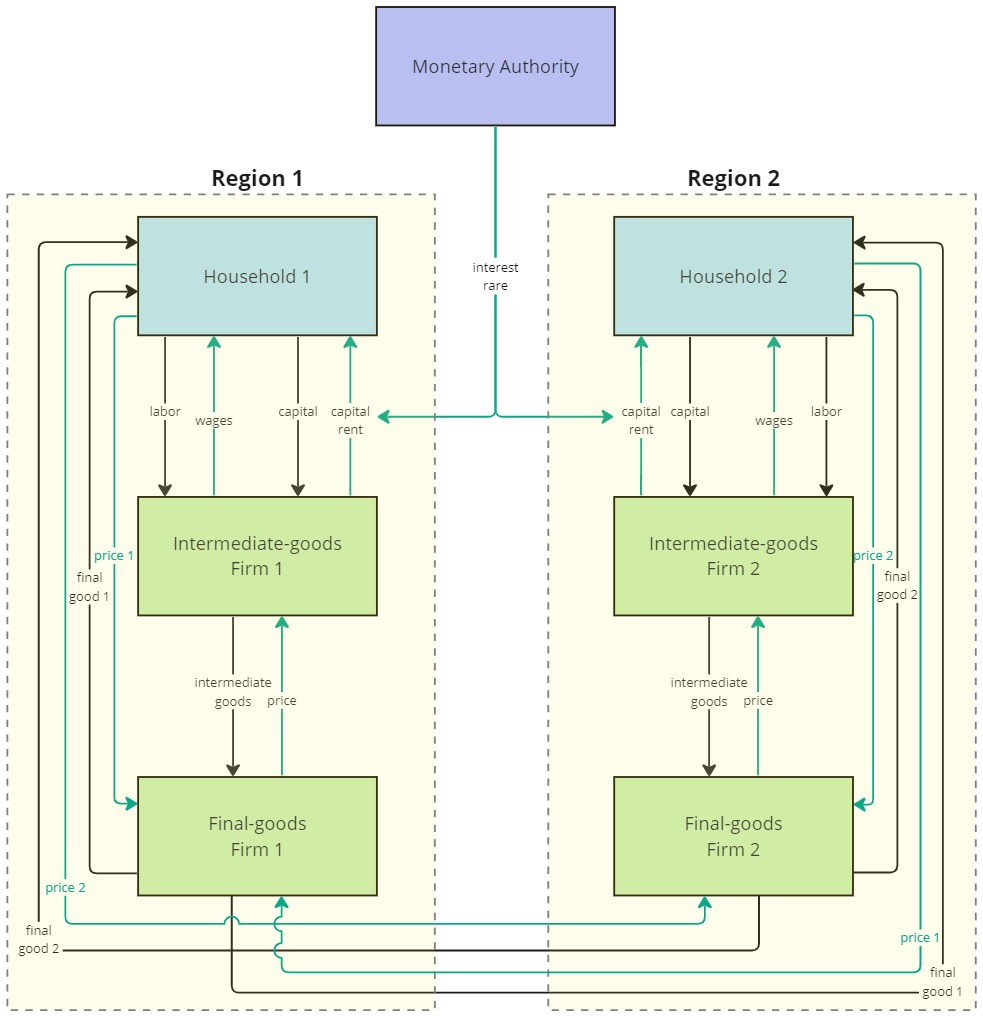
\includegraphics[width=\textwidth]{flowchart}
	\caption{Model Diagram}
	\label{fig:model-diagram}
\end{figure}

\newpage

% --------------------------------------------------
% REGIONAL MODEL
% --------------------------------------------------

% \subsubsection*{Regional Model}

% --------------------------------------------------
% HOUSEHOLD
% --------------------------------------------------

\subsubsection{Household}

\begin{tcolorbox}[colback=cyan!5!white,colframe=cyan!75!black]
	
	version 4: consumer price index instead of total expenses...
	
	sugestões do duplat e do matheus:
	
	- a inflação nacional ser a composição da inflação regional.
	
	- talvez o salário seja regional.
	
	- talvez a produtividade 2 seja uma proporção da primeira.
	
	- olhar as forward-looking variable(s) do modelo inicial.
	
\end{tcolorbox}

\subsubsection*{Utility Maximization Problem}

Following the models presented by \textcite{costa_junior_understanding_2016} and \textcite{solis-garcia_ucb_2022}, the representative household problem is to maximize an intertemporal utility function $U_{\eta}$ with respect to consumption $C_{\eta t}$ and labor $L_{\eta t}$, subject to a budget constraint, a capital accumulation rule and the non-negativity of real variables:
\begin{align}
	\max_{C_{\eta t}, L_{\eta t}, B_{\eta t}, K_{\eta, t+1}}: \quad & U_{\eta}(C_{\eta t},L_{\eta t}) = \E \sum_{t=0}^{\infty} \beta^t \left(\frac{C_{\eta t}^{1-\sigma}}{1-\sigma} - \phi \frac{L_{\eta t}^{1+\varphi}}{1+\varphi} \right) \label{eq:reg-utility-function-0} 
	\\
	\begin{split}
		\st: \quad & P_{1 t} C_{\eta 1 t} + P_{2 t} C_{\eta 2 t} + P_{\eta t} I_{\eta t} + B_{\eta t} = \\ & \quad = W_t L_{\eta t} + R_{Kt} K_{\eta t} + (1 + R_{t-1}) B_{\eta,t-1} + \Pi_{\eta t}
	\end{split} \label{eq:reg-budget-constraint} \\
	\quad & K_{\eta, t+1} = (1-\delta)K_{\eta t} + I_{\eta t} \label{eq:reg-law-of-motion-for-capital} \\
	\quad & C_{\eta t} = C_{\eta 1 t}^{\omega_{\eta 1}} C_{\eta 2 t}^{1-\omega_{\eta 1}} \label{eq:reg-consumption-aggregation} \\
	\quad & C_{\eta t}, L_{\eta t}, K_{\eta, t+1} > 0 \text{ ; $K_0$ given.} \nonumber
\end{align}

where $\E$ is the expectation operator, $\beta$ is the intertemporal discount factor, $\sigma$ is the relative risk aversion coefficient, $\phi$ is the relative labor weight in utility, $\varphi$ is the marginal disutility of labor supply. In the budget constraint, $P_{1t}$ and $P_{2t}$ are the prices of goods $1$ and $2$, respectively, $C_{\eta 1 t}$ and $C_{\eta 2 t}$ are the goods produced in region $1$ and $2$, respectively, and consumed in region $\eta$, $I_{\eta t}$ is the investment, $B_{\eta t}$ are the bonds, $W_t$ is the wage level, $K_{\eta t}$ is the capital, $R_{Kt}$ is the return on capital, $R_t$ is the return on bonds (which is also the nominal interest rate of the economy) and $\Pi_{\eta t}$ is the firm profit. In the capital accumulation rule, $\delta$ is the capital depreciation rate. In the consumption aggregation, ${\omega_{\eta 1}}$ and ${1 - \omega_{\eta 1}}$ are the weights of goods $C_{\eta 1 t}$ and $C_{\eta 2 t}$, respectively, in the consumption bundle $C_{\eta t}$.

To solve the household problem, first substitute \ref{eq:reg-consumption-aggregation} in \ref{eq:reg-utility-function-0}:
\begin{align}
	U_{\eta}(C_{\eta 1 t}, C_{\eta 2 t}, L_{\eta t}) = \E \sum_{t=0}^{\infty} \beta^t \left( \frac{\left[ C_{\eta 1 t}^{\omega_{\eta 1}} C_{\eta 2 t}^{1-\omega_{\eta 1}} \right]^{1-\sigma}}{1-\sigma} - \phi \frac{L_{\eta t}^{1+\varphi}}{1+\varphi} \right) \label{eq:reg-utility-function}
\end{align}

Isolate $I_{\eta t}$ in \ref{eq:reg-law-of-motion-for-capital} and substitute in \ref{eq:reg-budget-constraint}:
\begin{align}
	& K_{\eta, t+1} = (1-\delta)K_{\eta t} + I_{\eta t} \implies I_{\eta t} = K_{\eta, t+1} - (1-\delta)K_{\eta t} \tag{\ref{eq:reg-law-of-motion-for-capital}} \\
	\begin{split}
		& P_{1 t} C_{\eta 1 t} + P_{2 t} C_{\eta 2 t} + P_{\eta t} I_{\eta t} + B_{\eta t} = \\ & \quad = W_t L_{\eta t} + R_{Kt} K_{\eta t} + (1 + R_{t-1}) B_{\eta,t-1} + \Pi_{\eta t} \implies
	\end{split} \tag{\ref{eq:reg-budget-constraint}}
	\\
	\begin{split}
		& P_{1 t} C_{\eta 1 t} + P_{2 t} C_{\eta 2 t} + P_{\eta t} [ K_{\eta, t+1} - (1-\delta)K_{\eta t} ] + B_{\eta t} = \\ & \quad = W_t L_{\eta t} + R_{Kt} K_{\eta t} + (1 + R_{t-1}) B_{\eta,t-1} + \Pi_{\eta t}
	\end{split} \label{eq:reg-budget-constraint-2}
\end{align}

\subsubsection*{Lagrangian}

The maximization problem with restrictions can be transformed into one without restriction using the Lagrangian function $\mathcal{L}$ formed by \ref{eq:reg-utility-function} and \ref{eq:reg-budget-constraint-2}:
\begin{align}
	\begin{split}
	& \mathcal{L} = \mathbb{E}_t \sum_{t=0}^{\infty} \beta^t \left\{ \left( \frac{ \left[ C_{\eta 1 t}^{\omega_{\eta 1}} C_{\eta 2 t}^{1-\omega_{\eta 1}} \right]^{1 -\sigma}}{1 -\sigma} - \phi \frac{L_{\eta t}^{1+\varphi}}{1+\varphi} \right) \right. - \\ & \qquad - \mu_t \Big[ P_{1 t} C_{\eta 1 t} + P_{2 t} C_{\eta 2 t} + P_{\eta t} [ K_{\eta, t+1} - (1-\delta)K_{\eta t} ] + B_{\eta t} - \\ & \qquad \qquad \left. - ( W_t L_{\eta t} + R_{Kt} K_{\eta t} + (1 + R_{t-1}) B_{\eta,t-1} + \Pi_{\eta t} ) \Big] \right\} \label{eq:reg-household-lagrangian}
	\end{split}
\end{align}

\subsubsection*{First Order Conditions}

The first order conditions are:
\begin{align}
	C_{\eta 1 t}: \quad & \mu_t = \frac{\omega_{\eta 1} C_{\eta 1 t}^{\omega_{\eta 1} (1 -\sigma) -1} C_{\eta 2 t}^{(1 -\omega_{\eta 1})(1 -\sigma)}}{P_{1 t}} = \frac{\omega_{\eta 1}}{P_{1 t} C_{\eta 1 t}} C_{\eta t}^{1 -\sigma} \label{eq:reg-FOC-C1-eta-t} 
	\\
	C_{\eta 2 t}: \quad & \mu_t = \frac{(1 -\omega_{\eta 1}) C_{\eta 1 t}^{\omega_{\eta 1} (1 -\sigma)} C_{\eta 2 t}^{(1 -\omega_{\eta 1})(1 -\sigma)-1}}{P_{2 t}} = \frac{(1 -\omega_{\eta 1})}{P_{2 t} C_{\eta 2 t}} C_{\eta t}^{1 -\sigma} \label{eq:reg-FOC-C-2-eta-t} 
	\\
	L_{\eta t}: \quad & -\phi L_{\eta t}^{\varphi} +\mu_t W_t = 0 \implies \mu_t = \frac{\phi L_{\eta t}^{\varphi}}{W_t} \label{eq:reg-household-FOC-Lt} 
	\\
	\begin{split}
		B_{\eta t}: \quad & \beta^t \{-\mu_t\} + \E \beta^{t+1} \{ -\mu_{t+1} [-(1 + R_{t})] \} = 0 \implies \\ & \qquad \mu_t = \beta (1 + R_{t}) \E{ \mu_{t+1}}
	\end{split} \label{eq:reg-FOC-Bt}
	\\
	\begin{split}
		K_{\eta, t+1}: \quad & -\mu_t P_{\eta t} + \mathbb{E}_t \beta \{ \mu_{t+1} [(1-\delta) P_{\eta, t+1} + R_{K,t+1}] \} = 0 \implies \\ & \qquad \mu_t P_{\eta t} = \beta \mathbb{E}_t \{ \mu_{t+1} [(1-\delta) P_{\eta, t+1} + R_{K,t+1}] \}
	\end{split} \label{eq:reg-household-FOC-Kt} \\
	\begin{split}
		\mu_t: \quad & P_{1 t} C_{\eta 1 t} + P_{2 t} C_{\eta 2 t} + P_{\eta t} [ K_{\eta, t+1} - (1-\delta)K_{\eta t} ] + B_{\eta t} = \\ & \qquad = W_t L_{\eta t} + R_{Kt} K_{\eta t} + (1 + R_{t-1}) B_{\eta,t-1} + \Pi_{\eta t}
	\end{split} \tag{\ref{eq:reg-budget-constraint-2}}
\end{align}

\subsubsection*{Solutions}

Match \ref{eq:reg-FOC-C1-eta-t} and \ref{eq:reg-FOC-C-2-eta-t}:
\begin{align}
	& \mu_t = \frac{\omega_{\eta 1}}{P_{1 t} C_{\eta 1 t}} C_{\eta t}^{1 -\sigma} = \frac{(1 -\omega_{\eta 1})}{P_{2 t} C_{\eta 2 t}} C_{\eta t}^{1 -\sigma} \implies \nonumber \\
	& \frac{C_{\eta 1 t}}{C_{\eta 2 t}} = \frac{P_{2 t}}{P_{1 t}} \cdot \frac{\omega_{\eta 1}}{1 -\omega_{\eta 1}} \iff C_{\eta 1 t} = \frac{P_{2 t}}{P_{1 t}} \cdot \frac{\omega_{\eta 1}}{1 -\omega_{\eta 1}} \cdot C_{\eta 2 t} \label{eq:reg-FOC-C1-C2}
\end{align}

Equation \ref{eq:reg-FOC-C1-C2} is the relative consumption of regional goods in region $\eta$.

Substitute \ref{eq:reg-FOC-C1-C2} in \ref{eq:reg-consumption-aggregation}:
\begin{alignat}{2}
	C_{\eta t} &= C_{\eta 1 t}^{\omega_{\eta 1}} C_{\eta 2 t}^{1-\omega_{\eta 1}} &\implies \tag{\ref{eq:reg-consumption-aggregation}} \\
	C_{\eta t} &= \left[ \frac{P_{2 t}}{P_{1 t}} \cdot \frac{\omega_{\eta 1}}{1 -\omega_{\eta 1}} \cdot C_{\eta 2 t} \right]^{\omega_{\eta 1}} C_{\eta 2 t}^{1-\omega_{\eta 1}} &\implies \nonumber \\
	C_{\eta 2 t} &= C_{\eta t} \left[ \frac{P_{1 t}}{P_{2 t}} \cdot \frac{1 -\omega_{\eta 1}}{\omega_{\eta 1}} \right]^{\omega_{\eta 1}} \label{eq:reg-Cn-Cv}
\end{alignat}

Substitute \ref{eq:reg-Cn-Cv} in \ref{eq:reg-FOC-C1-C2}:
\begin{alignat}{2}
	C_{\eta 1 t} &= \frac{P_{2 t}}{P_{1 t}} \cdot \frac{\omega_{\eta 1}}{1 -\omega_{\eta 1}} \cdot C_{\eta 2 t} \tag{\ref{eq:reg-FOC-C1-C2}} &\implies \nonumber \\
	C_{\eta 1 t} &= \frac{P_{2 t}}{P_{1 t}} \cdot \frac{\omega_{\eta 1}}{1 -\omega_{\eta 1}} \cdot C_{\eta t} \left[ \frac{P_{1 t}}{P_{2 t}} \cdot \frac{1 -\omega_{\eta 1}}{\omega_{\eta 1}} \right]^{\omega_{\eta 1}} &\implies \nonumber \\
	C_{\eta 1 t} &= C_{\eta t} \left[ \frac{P_{1 t}}{P_{2 t}} \cdot \frac{1 -\omega_{\eta 1}}{\omega_{\eta 1}} \right]^{\omega_{\eta 1} -1} \label{eq:reg-Cn-Cn}
\end{alignat}

Define the total goods expense $\te$ of household $\eta$:
\begin{align}
	\te = P_{1 t} C_{\eta 1 t} + P_{2 t} C_{\eta 2 t} \label{eq:reg-total-expense}
\end{align}

Substitute \ref{eq:reg-Cn-Cv} and \ref{eq:reg-Cn-Cn} in \ref{eq:reg-total-expense}:
\begin{align}
	\te &= P_{1 t} C_{\eta t} \left[ \frac{P_{1 t}}{P_{2 t}} \cdot \frac{1 -\omega_{\eta 1}}{\omega_{\eta 1}} \right]^{\omega_{\eta 1} -1} + P_{2 t} C_{\eta t} \left[ \frac{P_{1 t}}{P_{2 t}} \cdot \frac{1 -\omega_{\eta 1}}{\omega_{\eta 1}} \right]^{\omega_{\eta 1}} \implies \nonumber \\
	\te &= C_{\eta t} \left[ \frac{P_{1 t}}{\omega_{\eta 1}} \right]^{\omega_{\eta 1}} \left[ \frac{P_{2 t}}{1 -\omega_{\eta 1}} \right]^{1 -\omega_{\eta 1}} \label{eq:reg-total-expense-level}
\end{align}

Equation \ref{eq:reg-total-expense-level} shows that the total expense with goods is proportional to the goods' prices $P_{1 t}$ and $P_{2 t}$.

Rewrite \ref{eq:reg-Cn-Cv} in terms of \ref{eq:reg-total-expense-level}:
\begin{alignat}{2}
	C_{\eta 2 t} &= C_{\eta t} \left[ \frac{P_{1 t}}{P_{2 t}} \cdot \frac{1 -\omega_{\eta 1}}{\omega_{\eta 1}} \right]^{\omega_{\eta 1}} &\implies \tag{\ref{eq:reg-Cn-Cv}} \\
	C_{\eta 2 t} &= C_{\eta t} \left[ \frac{P_{1 t}}{\omega_{\eta 1}} \right]^{\omega_{\eta 1}} \left[ \frac{P_{2 t}}{1 -\omega_{\eta 1}} \right]^{-\omega_{\eta 1}} \left[ \frac{P_{2 t}}{1 -\omega_{\eta 1}} \cdot \frac{1 -\omega_{\eta 1}}{P_{2 t}} \right] &\implies \nonumber \\
	C_{\eta 2 t} &= \te \frac{1 -\omega_{\eta 1}}{P_{2 t}} \label{eq:reg-Cn-Cv-2}
\end{alignat}

Rewrite \ref{eq:reg-Cn-Cn} in terms of \ref{eq:reg-total-expense-level} and isolate $(\sfrac{\omega_{\eta 1}}{P_{1 t} C_{\eta 1 t}})$:
	\begin{alignat}{2}
		C_{\eta 1 t} &= C_{\eta t} \left[ \frac{P_{1 t}}{P_{2 t}} \cdot \frac{1 -\omega_{\eta 1}}{\omega_{\eta 1}} \right]^{\omega_{\eta 1} -1} &\implies \tag{\ref{eq:reg-Cn-Cn}} \\
		C_{\eta 1 t} &= C_{\eta t} \left[ \frac{ P_{1 t}}{ \omega_{\eta 1}}\right]^{ \omega_{\eta 1}} \left[ \frac{P_{2 t}}{1-\omega_{\eta 1}} \right]^{1 -\omega_{\eta 1}} \left[ \frac{\omega_{\eta 1}}{P_{1 t}} \right] &\implies \nonumber \\
		C_{\eta 1 t} &= \te \frac{\omega_{\eta 1}}{P_{1 t}} \iff
		\frac{\omega_{\eta 1}}{P_{1 t} C_{\eta 1 t}} = \frac{1}{\te} \label{eq:reg-Cn-Cn-2}
	\end{alignat}

\begin{tcolorbox}[colback=red!5!white,colframe=red!75!black]

Divide \ref{eq:reg-Cn-Cn-2} by \ref{eq:reg-Cn-Cv-2}:
\begin{align}
	\frac{C_{\eta 1 t}}{C_{\eta 2 t}} &= \frac{\te \frac{\omega_{\eta 1}}{P_{1 t}}}{\te \frac{1 -\omega_{\eta 1}}{P_{2 t}}} \implies \nonumber \\
	\frac{P_{1 t} C_{\eta 1 t}}{\omega_{\eta 1}} &= \frac{P_{2 t} C_{\eta 2 t}}{1 -\omega_{\eta 1}} \label{eq:reg-Cn1-Cn2}
\end{align}

\end{tcolorbox}

Substitute \ref{eq:reg-Cn-Cn-2} in \ref{eq:reg-FOC-C1-eta-t}:
\begin{align}
	\mu_t &= \frac{\omega_{\eta 1}}{P_{1 t} C_{\eta 1 t}} C_{\eta t}^{1 -\sigma} \tag{\ref{eq:reg-FOC-C1-eta-t}} \implies \\
	\mu_t &= \frac{ C_{\eta t}^{1-\sigma}}{ \te}  \label{eq:reg-FOC-C1-eta-t2}
\end{align}

Match \ref{eq:reg-FOC-C1-eta-t2} and \ref{eq:reg-household-FOC-Lt}:
\begin{align}
	\mu_t = \frac{ C_{\eta t}^{1-\sigma}}{ \te} &= \frac{\phi L_{\eta t}^{\varphi}}{W_t} \implies \nonumber \\
	\frac{\phi L_{\eta t}^{\varphi}}{C_{\eta t}^{1-\sigma}} &= \frac{W_t}{\te} \label{eq:reg-labor-supply}
\end{align}

Equation \ref{eq:reg-labor-supply} is the Household Labor Supply and shows that the marginal rate of substitution (MRS) of labor for consumption is equal to the real wage, which is the relative price between labor and goods.

Substitute $\mu_t$ and $\mu_{t+1}$ from equation \ref{eq:reg-FOC-C1-eta-t2} in \ref{eq:reg-FOC-Bt}:
\begin{alignat}{2}
	\mu_t &= \beta (1 + R_{t}) \E{ \mu_{t+1}} &\implies \tag{\ref{eq:reg-FOC-Bt}} 
	\\
	\frac{ C_{\eta t}^{1-\sigma}}{ \te} &= \beta (1 + R_{t}) \E \left\{ \frac{ C_{\eta, t+1}^{1-\sigma}}{ \te[t+1]} \right\} \label{eq:reg-bonds-euler-equation}
\end{alignat}

Equation \ref{eq:reg-bonds-euler-equation} is the Euler equation for the bonds return.

Substitute $\mu_t$ and $\mu_{t+1}$ from equation \ref{eq:reg-FOC-C1-eta-t2} in \ref{eq:reg-household-FOC-Kt}:
\begin{alignat}{2}
	\mu_t P_{\eta t} &= \beta \mathbb{E}_t \{ \mu_{t+1} [(1-\delta) P_{\eta, t+1} + R_{K,t+1}] \} &\implies \tag{\ref{eq:reg-household-FOC-Kt}} 
	\\
	\frac{ C_{\eta t}^{1-\sigma}}{ \te} P_{\eta t} &= \beta \mathbb{E}_t \left\{ \frac{ C_{\eta, t+1}^{1-\sigma}}{ \te[t+1]} [(1-\delta) P_{\eta, t+1} + R_{K,t+1}] \right\} \label{eq:reg-capital-euler-equation}
\end{alignat}

Equation \ref{eq:reg-capital-euler-equation} is the Euler equation for the capital return.

% --------------------------------------------------
% FIRMS
% --------------------------------------------------

\subsubsection*{Firms}

Consider two types of firms: 
\begin{enumerate*}[label=(\arabic*)]
	\item a continuum of intermediate-goods firms, which operate in monopolistic competition and each produce one variety with imperfect substitution level between each other and
	
	\item the final-goods firm, which aggregates all the varieties into a final bundle and operates in perfect competition.
\end{enumerate*}

% --------------------------------------------------
% final-goods FIRM
% --------------------------------------------------

\subsubsection{Final-Goods Firm}

\subsubsection*{Profit Maximization Problem}

The role of the final-goods firm is to aggregate all the varieties $Y_{\eta jt}$ produced by the intermediate-goods firms in each region $\eta \in \{1,2\}$, so that the representative consumer can buy only one good $Y_{\eta t}$, the bundle good, from each region.

% The role of the final-goods firm is to aggregate all the varieties produced by the intermediate-goods firms, so that the representative consumer can buy only one good $Y_{\eta t}$, the bundle good.

% There are two regions and each region has a representative final-goods firm. The first region has a continuum of intermediate-goods firms indexes by $j \in [0,j_m]$ and the second region has firms indexed by $j \in \mathopen( j_m,1 \mathclose]$.\footnote{note that if $j_m > \sfrac{1}{2}$, then region $m$ is more industrious than region $m+1$.}

The final-goods firm problem is to maximize its profit, considering that its output is the bundle $Y_{\eta t}$ formed by a continuum $j \in [0,1]$ of intermediate goods $Y_{\eta jt}$, with elasticity of substitution between intermediate goods $\psi$:
\begin{align}
	\max_{Y_{\eta jt}}: &\quad \Pi_{\eta t} = P_{\eta t} Y_{\eta t} - \int_{0}^{1} P_{\eta jt} Y_{\eta jt} \dif j \label{eq:reg-final-goods-firm-max-problem} \\
	\st: & \quad Y_{\eta t} = \left( \int_{0}^{1} Y_{\eta jt}^{\frac{\psi-1}{\psi}} \dif j \right)^{\frac{\psi}{\psi-1}} \label{eq:reg-final-goods-firm-bundle-rule}
\end{align}

Substitute \ref{eq:reg-final-goods-firm-bundle-rule} in \ref{eq:reg-final-goods-firm-max-problem}:
\begin{align}
	\label{eq:reg-final-goods-firm-max-problem-2}
	\max_{Y_{\eta jt}}: & \quad \Pi_{\eta t} = P_{\eta t} \left( \int_{0}^{1} Y_{\eta jt}^{\frac{\psi-1}{\psi}} \dif j \right)^{\frac{\psi}{\psi-1}} - \int_{0}^{1} P_{\eta jt} Y_{\eta jt} \dif j
\end{align}

\subsubsection*{First Order Condition and Solutions}

The first order condition is:
\begin{align}
	Y_{\eta jt}:\quad & P_{\eta t} \left( \frac{\psi}{\psi-1} \right) \left( \int_{0}^{1} Y_{\eta jt}^{\frac{\psi-1}{\psi}} \dif j \right)^{\frac{\psi}{\psi-1}-1} \left( \frac{\psi-1}{\psi} \right) Y_{\eta jt}^{\frac{\psi-1}{\psi}-1} - P_{\eta jt} = 0 \implies \nonumber \\
	\label{eq:reg-final-goods-firm-FOC}
	& Y_{\eta jt} = Y_{t} \left( \frac{P_{\eta t}}{P_{\eta jt}} \right)^{\psi}
\end{align}

Equation \ref{eq:reg-final-goods-firm-FOC} shows that the demand for variety $j$ depends on its relative price. 

Substitute \ref{eq:reg-final-goods-firm-FOC} in \ref{eq:reg-final-goods-firm-bundle-rule}:
\begin{alignat}{2}
	Y_{\eta t} & = \left( \int_{0}^{1} Y_{\eta jt}^{\frac{\psi-1}{\psi}} \dif j \right)^{\frac{\psi}{\psi-1}} &\implies \nonumber \\
	Y_{\eta t} & = \left( \int_{0}^{1} \left[ Y_{\eta t} \left( \frac{P_{\eta t}}{P_{\eta jt}} \right)^{\psi} \right]^{\frac{\psi-1}{\psi}} \dif j \right)^{\frac{\psi}{\psi-1}} \quad &\implies \nonumber \\
	P_{\eta t} & = \left[ \int_{0}^{1} P_{\eta jt}^{1-\psi} \dif j \right]^{\frac{1}{1-\psi}} \label{eq:reg-final-goods-firm-markup}
\end{alignat}

Equation \ref{eq:reg-final-goods-firm-markup} is the final-goods firm's markup.

% --------------------------------------------------
% intermediate-goods FIRM
% --------------------------------------------------

\subsubsection{Intermediate-Goods Firms}

\subsubsection*{Cost Minimization Problem}

The intermediate-goods firms, denoted by $j \in [0,1]$, produce varieties of a representative good with a certain level of substitutability. Each of these firms has to choose capital $K_{\eta jt}$ and labor $L_{\eta jt}$ to minimize production costs, subject to a technology rule.
\begin{align}
	\label{eq:reg-int-good-firm-total-cost}
	\min_{K_{\eta jt}, L_{\eta jt}}: \quad & R_{Kt} K_{\eta jt} + W_t L_{\eta jt} \\
	\label{eq:reg-int-good-firm-production-function}
	\st: \quad & Y_{\eta jt} = Z_{A\eta t} K_{\eta jt}^{\alpha_{\eta}} L_{\eta jt}^{1-{\alpha_{\eta}}}
\end{align}

where $Y_{\eta jt}$ is the output obtained by the production technology level $Z_{A\eta t}$ that transforms capital $K_{\eta jt}$ and labor $L_{\eta jt}$ in proportions ${\alpha_{\eta}}$ and $(1-{\alpha_{\eta}})$, respectively, into intermediate goods.\footnote{the production technology level $Z_{A\eta t}$ will be submitted to a productivity shock, detailed in section \ref{sec:reg-productivity-shock}.}

\subsubsection*{Lagrangian}

Transform the minimization problem with restriction into one without restriction applying the Lagrangian function $\mathcal{L}$:
\begin{align}
	\label{eq:reg-int-good-firm-lagrangian}
	\mathcal{L} = (R_{Kt} K_{\eta jt} + W_t L_{\eta jt}) - \Lambda_{\eta jt} (Z_{A\eta t} K_{\eta jt}^{\alpha_{\eta}} L_{\eta jt}^{1-{\alpha_{\eta}}} - Y_{\eta jt})
\end{align}

where the Lagrangian multiplier $\Lambda_{\eta jt}$ is the marginal cost.\footnote{see Lemma \ref{lemma:marginal-cost}}

\subsubsection*{First Order Conditions}

The first-order conditions are:
\begin{alignat}{2}
	K_{\eta jt}: \quad & R_{Kt} - \Lambda_{\eta jt} Z_{A\eta t} {\alpha_{\eta}} K_{\eta jt}^{{\alpha_{\eta}}-1} L_{\eta jt}^{1-{\alpha_{\eta}}} = 0 &&\implies \nonumber \\
	& K_{\eta jt} = {\alpha_{\eta}} Y_{\eta jt} \frac{\Lambda_{\eta jt}}{R_{Kt}} \label{eq:reg-int-good-firm-FOC-Kt} \\
	L_{\eta jt}: \quad & W_t - \Lambda_{\eta jt} Z_{A\eta t} K_{\eta jt}^{\alpha_{\eta}} (1-{\alpha_{\eta}}) L_{\eta jt}^{-{\alpha_{\eta}}} = 0 \quad &&\implies \nonumber \\ 
	& L_{\eta jt} = (1-{\alpha_{\eta}}) Y_{\eta jt} \frac{\Lambda_{\eta jt}}{W_t} \label{eq:reg-int-good-firm-FOC-Lt} \\
	\Lambda_{\eta jt}: \quad & Y_{\eta jt} = Z_{A\eta t} K_{\eta jt}^{\alpha_{\eta}} L_{\eta jt}^{1-{\alpha_{\eta}}} \tag{\ref{eq:reg-int-good-firm-production-function}}
\end{alignat}

\subsubsection*{Solutions}

Divide equation \ref{eq:reg-int-good-firm-FOC-Kt} by \ref{eq:reg-int-good-firm-FOC-Lt}:
\begin{align}
	\frac{K_{\eta jt}}{L_{\eta jt}} = \frac{{\alpha_{\eta}} Y_{\eta jt} \Lambda_{\eta jt} /R_{Kt}}{(1-{\alpha_{\eta}}) Y_{\eta jt} \Lambda_{\eta jt} /W_t} \implies
	\frac{K_{\eta jt}}{L_{\eta jt}} = \left( \frac{{\alpha_{\eta}}}{1-{\alpha_{\eta}}} \right) \frac{W_t}{R_{Kt}} \label{eq:reg-int-good-firm-TMRS}
\end{align}

Equation \ref{eq:reg-int-good-firm-TMRS} demonstrates the relationship between the technical marginal rate of substitution (TMRS) and the economical marginal rate of substitution (EMRS). 

Substitute $L_{\eta jt}$ from equation \ref{eq:reg-int-good-firm-TMRS} in \ref{eq:reg-int-good-firm-production-function}:
\begin{alignat}{2}
	Y_{\eta jt} & = Z_{A\eta t} K_{\eta jt}^{\alpha_{\eta}} L_{\eta jt}^{1-{\alpha_{\eta}}} &\implies \nonumber \\
	Y_{\eta jt} & = Z_{A\eta t} K_{\eta jt}^{\alpha_{\eta}} \left[ \left( \frac{1-{\alpha_{\eta}}}{{\alpha_{\eta}}} \right) \frac{R_{Kt} K_{\eta jt}}{W_t} \right]^{1-{\alpha_{\eta}}} &\implies \nonumber \\
	K_{\eta jt} & = \frac{Y_{\eta jt}}{Z_{A\eta t}} \left[ \left( \frac{{\alpha_{\eta}}}{1-{\alpha_{\eta}}} \right) \frac{W_t}{R_{Kt}}\right]^{1-{\alpha_{\eta}}} \label{eq:reg-int-good-firm-Kt-demand}
\end{alignat}

Equation \ref{eq:reg-int-good-firm-Kt-demand} is the intermediate-goods firm demand for capital. 

Substitute \ref{eq:reg-int-good-firm-Kt-demand} in \ref{eq:reg-int-good-firm-TMRS}:
\begin{alignat}{2}
	L_{\eta jt} & = \left( \frac{1-{\alpha_{\eta}}}{{\alpha_{\eta}}} \right) \frac{R_{Kt} K_{\eta jt}}{W_t} &\implies \nonumber \\
	L_{\eta jt} & = \left( \frac{1-{\alpha_{\eta}}}{{\alpha_{\eta}}} \right) \frac{R_{Kt}}{W_t} \frac{Y_{\eta jt}}{Z_{A\eta t}} \left[ \left( \frac{{\alpha_{\eta}}}{1-{\alpha_{\eta}}} \right) \frac{W_t}{R_{Kt}}\right]^{1-{\alpha_{\eta}}} &\implies \nonumber \\
	L_{\eta jt} & = \frac{Y_{\eta jt}}{Z_{A\eta t}} \left[ \left( \frac{{\alpha_{\eta}}}{1-{\alpha_{\eta}}} \right) \frac{W_t}{R_{Kt}}\right]^{-{\alpha_{\eta}}} \label{eq:reg-int-good-firm-Lt-demand}
\end{alignat}

Equation \ref{eq:reg-int-good-firm-Lt-demand} is the intermediate-goods firm demand for labor.

\subsubsection*{Total and Marginal Costs}

Calculate the total cost $TC$ using \ref{eq:reg-int-good-firm-Kt-demand} and \ref{eq:reg-int-good-firm-Lt-demand}:
\begin{alignat}{2}
	TC_{\eta jt} & = W_t L_{\eta jt} + R_{Kt} K_{\eta jt} &\implies \nonumber \\
	TC_{\eta jt} & = W_t \frac{Y_{\eta jt}}{Z_{A\eta t}} \left[ \left( \frac{{\alpha_{\eta}}}{1-{\alpha_{\eta}}} \right) \frac{W_t}{R_{Kt}} \right]^{-{\alpha_{\eta}}} + R_{Kt} \frac{Y_{\eta jt}}{Z_{A\eta t}} \left[ \left( \frac{{\alpha_{\eta}}}{1-{\alpha_{\eta}}} \right) \frac{W_t}{R_{Kt}} \right]^{1-{\alpha_{\eta}}} &\implies \nonumber \\
	TC_{\eta jt} & = \frac{Y_{\eta jt}}{Z_{A\eta t}} \left( \frac{R_{Kt}}{{\alpha_{\eta}}} \right)^{{\alpha_{\eta}}} \left( \frac{W_t}{1-{\alpha_{\eta}}} \right)^{1-{\alpha_{\eta}}} \label{eq:reg-int-good-firm-TC}
\end{alignat}

%%%%%

Calculate the marginal cost $\Lambda$ using \ref{eq:reg-int-good-firm-TC}: 
\begin{align}
	\Lambda_{\eta jt} & = \frac{\partial TC_{\eta jt}}{\partial Y_{\eta jt}} \implies 
	\Lambda_{\eta jt} = \frac{1}{Z_{A\eta t}} \left( \frac{R_{Kt}}{{\alpha_{\eta}}} \right)^{{\alpha_{\eta}}} \left( \frac{W_t}{1-{\alpha_{\eta}}} \right)^{1-{\alpha_{\eta}}} \label{eq:reg-int-good-firm-MC}
\end{align}

The marginal cost depends on the technological level $Z_{A\eta t}$, the nominal interest rate $R_{Kt}$ and the nominal wage level $W_t$, which are the same for all intermediate-goods firms, and because of that, the index $j$ may be dropped:
\begin{align}
	\label{eq:reg-int-good-firm-MC-2}
	\Lambda_{\eta t} = \frac{1}{Z_{A\eta t}} \left( \frac{R_{Kt}}{{\alpha_{\eta}}} \right)^{{\alpha_{\eta}}} \left( \frac{W_t}{1-{\alpha_{\eta}}} \right)^{1-{\alpha_{\eta}}}
\end{align}

notice that:
\begin{align}
	\label{eq:reg-int-good-firm-TC-MC}
	\Lambda_{\eta t} = \frac{TC_{\eta jt}}{Y_{\eta jt}} \implies 
	TC_{\eta jt} = \Lambda_{\eta t} Y_{\eta jt}
\end{align}

% --------------------------------------------------
% CALVO RULE
% --------------------------------------------------

\subsubsection*{Optimal Price Problem}

Consider an economy with price stickiness, following the Calvo Rule \cite{calvo_staggered_1983}: each firm has a probability $(0 < \theta < 1)$ of keeping its price in the next period ($P_{\eta j,t+1} = P_{\eta jt}$), and a probability of $(1 - \theta)$ of setting a new optimal price $P_{\eta jt}^{\ast}$ that maximizes its profits. Therefore, each firm must take this uncertainty into account when deciding the optimal price: the intertemporal profit flow, given the nominal interest rate $R_{t}$ of each period, is calculated considering the probability $\theta$ of keeping the previous price.

\begin{align}
	\label{eq:reg-int-good-firm-optimal-price-problem}
	\max_{P_{\eta jt}}: & \quad \E \sum_{s=0}^{\infty} \left\{ \frac{ \theta^s \left[ P_{\eta jt} Y_{\eta j,t+s} - TC_{\eta j,t+s} \right]}{\prod_{k=0}^{s-1}(1+R_{t+k})} \right\} \\
	\tag{\ref{eq:reg-final-goods-firm-FOC}}
	\st: & \quad Y_{\eta jt} = Y_{\eta t} \left( \frac{P_{\eta t}}{P_{\eta jt}} \right)^{\psi}
\end{align}

%%%%%

Substitute \ref{eq:reg-int-good-firm-TC-MC} in \ref{eq:reg-int-good-firm-optimal-price-problem}:
\begin{align}
	\label{eq:reg-int-good-firm-optimal-price-problem-2}
	\max_{P_{\eta jt}}: & \quad \E \sum_{s=0}^{\infty} \left\{ \frac{\theta^s \big[ P_{\eta jt} Y_{\eta j,t+s} - \Lambda_{\eta, t+s} Y_{\eta j,t+s} \big]}{\prod_{k=0}^{s-1}(1+R_{t+k})} \right\}
\end{align}

Substitute \ref{eq:reg-final-goods-firm-FOC} in \ref{eq:reg-int-good-firm-optimal-price-problem-2} and rearrange the variables:
\begin{align}
	\max_{P_{\eta jt}}: & \quad \E \sum_{s=0}^{\infty} \left\{ \frac{\theta^s \left[ P_{\eta jt} Y_{\eta t+s} \left( \frac{P_{\eta, t+s}}{P_{\eta jt}} \right)^{\psi} - \Lambda_{\eta, t+s} Y_{\eta t+s} \left( \frac{P_{\eta, t+s}}{P_{\eta jt}} \right)^{\psi} \right]}{\prod_{k=0}^{s-1}(1+R_{t+k})} \right\} \implies \nonumber 
	\\
	\max_{P_{\eta jt}}: & \quad \E \sum_{s=0}^{\infty} \left\{ \frac{\theta^s \left[ P_{\eta jt}^{1-\psi} P_{\eta, t+s}^{\psi} Y_{\eta t+s} - P_{\eta jt}^{-\psi} P_{\eta, t+s}^{\psi} Y_{\eta t+s} \Lambda_{\eta, t+s} \right]}{\prod_{k=0}^{s-1}(1+R_{t+k})} \right\} \nonumber
\end{align}

%%%%%

\subsubsection*{First Order Condition}

The first order condition with respect to $P_{\eta jt}$ is:
\begin{align}
	& \quad \E \sum_{s=0}^{\infty} \left\{ \frac{\theta^s \left[ (1-\psi) P_{\eta jt}^{-\psi} P_{\eta, t+s}^{\psi} Y_{\eta t+s} - (-\psi) P_{\eta jt}^{-\psi-1} P_{\eta, t+s}^{\psi} Y_{\eta t+s} \Lambda_{\eta, t+s} \right]}{\prod_{k=0}^{s-1}(1+R_{t+k})} \right\} = 0 \nonumber
\end{align}

%%%%%

Separate the summations and rearrange the variables:
\begin{align}
	\begin{split}
		\E \sum_{s=0}^{\infty} &\left\{ \frac{\theta^s (\psi-1) \left( \frac{P_{\eta, t+s}} {P_{\eta jt}} \right)^{\psi} Y_{\eta t+s}} {\prod_{k=0}^{s-1} (1+R_{t+k})} \right\} = \\
		&= \E \sum_{s=0}^{\infty} \left\{ \frac{\theta^s \psi P_{\eta jt}^{-1} \left( \frac{P_{\eta, t+s}} {P_{\eta jt}} \right)^{\psi} Y_{\eta t+s} \Lambda_{\eta, t+s}}{\prod_{k=0}^{s-1}(1+R_{t+k})} \right\} \label{eq:reg-int-good-firm-optimal-price-FOC}
	\end{split}
\end{align}

%%%%%

Substitute \ref{eq:reg-final-goods-firm-FOC} in \ref{eq:reg-int-good-firm-optimal-price-FOC}:
\begin{alignat}{2}
	\E \sum_{s=0}^{\infty} \Bigg\{ \frac{\theta^s (\psi-1) Y_{\eta j,t+s}}{\prod_{k=0}^{s-1}(1+R_{t+k})} \Bigg\} &= \E \sum_{s=0}^{\infty} \Bigg\{ \frac{\theta^s \psi P_{\eta jt}^{-1} Y_{\eta j,t+s} \Lambda_{\eta, t+s}}{\prod_{k=0}^{s-1}(1+R_{t+k})}  \Bigg\} &\implies \nonumber \\
	(\psi-1) \E \sum_{s=0}^{\infty} \Bigg\{ \frac{\theta^s Y_{\eta j,t+s}}{\prod_{k=0}^{s-1}(1+R_{t+k})} \Bigg\} &= \psi P_{\eta jt}^{-1} \E \sum_{s=0}^{\infty} \Bigg\{ \frac{\theta^s Y_{\eta j,t+s} \Lambda_{\eta, t+s}}{\prod_{k=0}^{s-1}(1+R_{t+k})}  \Bigg\} &\implies \nonumber \\
	P_{\eta jt} \E \sum_{s=0}^{\infty} \Bigg\{ \frac{\theta^s Y_{\eta j,t+s}}{\prod_{k=0}^{s-1}(1+R_{t+k})} \Bigg\} &= \frac{\psi}{\psi-1} \E \sum_{s=0}^{\infty} \Bigg\{ \frac{\theta^s Y_{\eta j,t+s} \Lambda_{\eta, t+s}}{\prod_{k=0}^{s-1}(1+R_{t+k})}  \Bigg\} &\implies \nonumber
\end{alignat}

\vspace*{-1cm}

\begin{align}
	\label{eq:reg-int-good-firm-optimal-price-FOC-2}
	P_{\eta jt}^{\ast} &= 
	\frac{\psi}{\psi-1} \cdot
	\frac{
		\E \sum_{s=0}^{\infty} \left\{ 
		\theta^s Y_{\eta j,t+s} \Lambda_{\eta, t+s} / \prod_{k=0}^{s-1}(1+R_{t+k}) \right\}} {\E \sum_{s=0}^{\infty} \left\{
		\theta^s Y_{\eta j,t+s} / \prod_{k=0}^{s-1}(1+R_{t+k}) \right\}}
\end{align}

%%%%%

Equation \ref{eq:reg-int-good-firm-optimal-price-FOC-2} represents the optimal price that firm $j$ will choose. Since all firms that are able to choose will opt for the highest possible price, they will all select the same price. As a result, the index $j$ can be omitted:
\begin{align}
	\label{eq:reg-int-good-firm-optimal-price-FOC-3}
	P_{\eta t}^{\ast} &= 
	\frac{\psi}{\psi-1} \cdot
	\frac{
		\E \sum_{s=0}^{\infty} \left\{ 
		\theta^s Y_{\eta j,t+s} \Lambda_{\eta, t+s} / \prod_{k=0}^{s-1}(1+R_{t+k}) \right\}} {\E \sum_{s=0}^{\infty} \left\{
		\theta^s Y_{\eta j,t+s} / \prod_{k=0}^{s-1}(1+R_{t+k}) \right\}}
\end{align}

% --------------------------------------------------
% final-goods FIRM, PART II
% --------------------------------------------------

\subsubsection*{Final-Goods Firm, part II}

The process of fixing prices is random: in each period, $\theta$ firms will maintain the price from the previous period, while $(1-\theta)$ firms will choose a new optimal price. The price level for each period will be a composition of these two prices. Use this information in \ref{eq:reg-final-goods-firm-markup} to determine the aggregate price level:
\begin{align}
	P_{\eta t} & = \left[ \int_{0}^{\theta} P_{\eta, t-1}^{1-\psi} \dif j + \int_{\theta}^{1} P_{\eta t}^{\ast 1-\psi} \dif j \right]^{\frac{1}{1-\psi}}  \implies \nonumber \\
	P_{\eta t} & = \left[ \theta P_{\eta, t-1}^{1-\psi} + (1-\theta) P_{\eta t}^{\ast 1-\psi} \right]^\frac{1}{1-\psi} \label{eq:reg-general-price-level}
\end{align}

Equation \ref{eq:reg-general-price-level} is the aggregate price level.

% --------------------------------------------------
% MONETARY AUTHORITY
% --------------------------------------------------

\subsubsection{Monetary Authority}

The objective of the monetary authority is to conduct the economy to price stability and economic growth, using a Taylor rule \cite{taylor_discretion_1993} to determine the nominal interest rate:
\begin{align}
	\label{eq:reg-monetary-policy}
	\frac{R_{t}}{R} =
	\left( \frac{R_{t-1}}{R} \right)^{\gamma_R}  \left[
	\left( \frac{\pi_t}{\pi} \right)^{\gamma_\pi}
	\left( \frac{Y_{t}}{Y} \right)^{\gamma_Y} \right]^{1-\gamma_R} Z_{Mt}
\end{align}

where $R, \pi, Y$ are the variables in steady state, $\gamma_R$ is the smoothing parameter for the interest rate $R_{Kt}$, $\gamma_\pi$ and $\gamma_Y$ are the interest-rate sensitivities in relation to inflation and product, respectively, $Z_{Mt}$ is the monetary shock and $\pi_t$ is the gross inflation rate, defined by:\footnote{for the monetary shock definition, see section \ref{sec:reg-monetary-shock}.}
\begin{align}
	\pi_t = \frac{P_t}{P_{t-1}}
	\label{eq:reg-gross-inflation-rate}
\end{align}

where $P_t$ is the national price level, defined by:
\begin{align}
	P_{t} Y_{t} &= P_{1t} Y_{1t} + P_{2t} Y_{2t} \iff P_{t} = \frac{P_{1t} Y_{1t} + P_{2t} Y_{2t}}{Y_{t}} \label{eq:national-price-level}
\end{align}

\begin{comment}
	\begin{align}
		P_{t} Y_{t} &= P_{1t} Y_{1t} + P_{2t} Y_{2t} \implies \nonumber \\
		P_{t} &= \frac{Y_{1t}}{Y_{t}} P_{1t} + \frac{Y_{2t}}{Y_{t}} P_{2t} \implies \nonumber \\
		P_{t} &= \theta_{P1} P_{1t} + (1 -\theta_{P1}) P_{2t} %\label{eq:national-price-level}
	\end{align}
	
	where $\theta_{P1}$ and $(1-\theta_{P1})$ are the price level weights of regions 1 and 2 in the national price level composition, respectively:
	\begin{align}
		\left\langle \begin{matrix} \theta_{P1} & (1-\theta_{P1}) \end{matrix} \right\rangle \coloneq \left\langle \begin{matrix} \frac{Y_{1t}}{Yt} & \frac{Y_{2t}}{Yt} \end{matrix} \right\rangle \label{eq:reg-ss-P1-P2-weight-in-P}
	\end{align}
\end{comment}

\subsubsection*{Regional Inflation}

There is one price level $P_{\eta t}$ in each region, generating a regional inflation rate:
\begin{align}
	\pi_{\eta t} = \frac{P_{\eta t}}{P_{\eta, t-1}} \label{eq:regional-inflation}
\end{align}

% --------------------------------------------------
% STOCHASTIC SHOCKS
% --------------------------------------------------

\subsubsection{Stochastic Shocks}\label{sec:reg-stochastic-shocks}

\subsubsection*{Productivity Shock} \label{sec:reg-productivity-shock}

The production technology level $Z_{A\eta t}$ will be submitted to a productivity shock defined by a first-order autoregressive process $AR(1)$:
\begin{align}
	\ln{Z_{A\eta t}} = (1-\rho_{A\eta})\ln{Z_{A\eta}} + \rho_{A\eta}\ln{Z_{A\eta,t-1}} + \varepsilon_{A\eta t} \label{eq:reg-productivity-shock}
\end{align}

where $\rho_{A\eta} \in [0,1]$ and $\varepsilon_{A\eta t} \sim \mathscr{N}(0,\sigma_{A\eta})$.

\subsubsection*{Monetary Shock} \label{sec:reg-monetary-shock}

The monetary policy will also be submitted to a shock, through the variable $Z_{Mt}$, defined by a first-order autoregressive process $AR(1)$:
\begin{align}
	\ln{Z_{Mt}} = (1-\rho_M)\ln{Z_{M}} + \rho_M\ln{Z_{M,t-1}} + \varepsilon_{Mt} \label{eq:reg-monetary-shock}
\end{align}

where $\rho_M \in [0,1]$ and $\varepsilon_{Mt} \sim \mathscr{N}(0,\sigma_M)$.

% --------------------------------------------------
% EQUILIBRIUM CONDITIONS
% --------------------------------------------------

\subsubsection{Equilibrium Conditions}

% removed from the household solution set: I_{\eta t}^{\ast}, 

A Competitive Equilibrium consists of sequences of prices $\{P_{\eta t}^{\ast}, R_t^{\ast}, R_{Kt}^{\ast}, W_t^{\ast}\}$, allocations for households $\mathbfscr{A}_H \coloneq \{C_{\eta 1 t}^{\ast}, C_{\eta 2 t}^{\ast}, L_{\eta t}^{\ast}, B_{\eta t}^{\ast}, K_{\eta, t+1}^{\ast}\}$ and allocations  for firms $\mathbfscr{A}_F \coloneq \{K_{\eta jt}^{\ast}, L_{\eta jt}^{\ast}, Y_{\eta jt}^{\ast}, Y_{\eta t}^{\ast}\}$. In such an equilibrium, given the set of exogenous variables $\{K_0, Z_{A\eta t}, Z_{Mt}\}$, the elements in $\mathbfscr{A}_H$ solve the household problem, while the elements in $\mathbfscr{A}_F$ solve the firms' problems, and the markets for goods and labor clear:
\begin{tcolorbox}[colback=red!5!white,colframe=red!75!black]
	
	\begin{align}
		Y_{t} &= Y_{1 t} + Y_{2 t} \label{eq:reg-market-clearing-condition-Yt} \\
		& \text{where:} \quad Y_{\eta t} = C_{\eta t} + I_{\eta t} \label{eq:reg-regional-demand} \\
		L_{\eta t} &= \int_{0}^{1} L_{\eta jt} \: \dif \! j \label{eq:reg-market-clearing-condition-Lt}
	\end{align}
	
\end{tcolorbox}

\begin{comment}

\begin{align}
	Y_{t} &= Y_{1 t} + Y_{2 t} \label{eq:reg-market-clearing-condition-Yt} \\
	& \text{where:} \quad Y_{\eta t} = C_{\eta 1 t} + C_{\eta 2 t} + I_{\eta t} \label{eq:reg-regional-demand} \\
	L_{\eta t} &= \int_{0}^{1} L_{\eta jt} \dif j \label{eq:reg-market-clearing-condition-Lt}
\end{align}

\end{comment}

% \newpage

% --------------------------------------------------
% MODEL STRUCTURE
% --------------------------------------------------

\subsubsection{Model Structure}

The model is composed of the preview solutions, forming a square system of 41 variables and 41 equations, summarized as follows:

{\singlespacing
	
	\begin{itemize}

		\item Variables:
		
	\begin{itemize}
	
		\item from the household problem: $\langle \begin{smallmatrix} C_{\eta t} & L_{\eta t} & B_{\eta t} & K_{\eta, t+1} & C_{\eta 1t} & C_{\eta 2t} & \te \end{smallmatrix} \rangle$;
		
		\item from the final-goods firm problem: $\langle \begin{smallmatrix} Y_{\eta jt} & Y_{\eta t} & P_{\eta t} \end{smallmatrix} \rangle$;

		\item from the intermediate-goods firm problems: $\langle \begin{smallmatrix} K_{\eta jt} & L_{\eta jt} & P_{\eta t}^{\ast} \end{smallmatrix} \rangle$;
		
		\item from the monetary policy: $\langle \begin{smallmatrix} R_{t} & \pi_{t} & Y_{t} \end{smallmatrix} \rangle$;
		
		\item from the market clearing condition: $\langle \begin{smallmatrix} I_{\eta t} \end{smallmatrix} \rangle$;
		
		\item prices: $\langle \begin{smallmatrix} W_{t} & R_{Kt} & \Lambda_{\eta t} & P_{t} & \pi_{\eta t} \end{smallmatrix} \rangle$;
		
		\item shocks: $\langle \begin{smallmatrix} Z_{A\eta t} & Z_{Mt} \end{smallmatrix} \rangle$.

	\end{itemize}

		\item Equations:
		
	\begin{enumerate}

		\item Budget Constraint:
		\begin{align}
		\begin{split}
			& P_{1 t} C_{\eta 1 t} + P_{2 t} C_{\eta 2 t} + P_{\eta t} I_{\eta t} + B_{\eta t} = \\ & \quad = W_t L_{\eta t} + R_{Kt} K_{\eta t} + (1 + R_{t-1}) B_{\eta,t-1} + \Pi_{\eta t}
		\end{split} \tag{\ref{eq:reg-budget-constraint}}
		\end{align}

		\item Law of Motion for Capital:
		\begin{align}
			K_{\eta, t+1} = (1-\delta)K_{\eta t} + I_{\eta t} \tag{\ref{eq:reg-law-of-motion-for-capital}}
		\end{align}
	
		\begin{tcolorbox}[colback=red!5!white,colframe=red!75!black]
		
		\item Regional Consumption:
		\begin{align}
			C_{\eta t} &= C_{\eta 1 t}^{\omega_{\eta 1}} C_{\eta 2 t}^{1-\omega_{\eta 1}} \tag{\ref{eq:reg-consumption-aggregation}} 
		\end{align}
			
		\item Regional Expense Weight:
		\begin{align}
			\frac{P_{1 t} C_{\eta 1 t}}{\omega_{\eta 1}} &= \frac{P_{2 t} C_{\eta 2 t}}{1 -\omega_{\eta 1}} \tag{\ref{eq:reg-Cn1-Cn2}}
		\end{align}
		
		\begin{comment}
			
			\item Regional Consumption of good 1:
			\begin{align}
				C_{\eta 1 t} &= \te \frac{\omega_{\eta 1}}{P_{1 t}} \tag{\ref{eq:reg-Cn-Cn-2}}
			\end{align}
			
			\item Regional Consumption of good 2:
			\begin{align}
				C_{\eta 2 t} &= \te \frac{1 -\omega_{\eta 1}}{P_{2 t}} \tag{\ref{eq:reg-Cn-Cv-2}}
			\end{align}
			
		\end{comment}
				
		\end{tcolorbox}

		\item Price Composition of Consumption Bundle:
		\begin{align}
			\te &= C_{\eta t} \left[ \frac{P_{1 t}}{\omega_{\eta 1}} \right]^{\omega_{\eta 1}} \left[ \frac{P_{2 t}}{1 -\omega_{\eta 1}} \right]^{1 -\omega_{\eta 1}} \tag{\ref{eq:reg-total-expense-level}}
		\end{align}

		\item Labor Supply:
		\begin{align}
			\frac{\phi L_{\eta t}^{\varphi}}{C_{\eta t}^{1-\sigma}} = \frac{W_t}{\te} \tag{\ref{eq:reg-labor-supply}}
		\end{align}

		\item Euler equation for the bonds return:
		\begin{align}
			\frac{ C_{\eta t}^{1-\sigma}}{ \te} &= \beta (1 + R_{t}) \E \left\{ \frac{ C_{\eta, t+1}^{1-\sigma}}{ \te[t+1]} \right\} \tag{\ref{eq:reg-bonds-euler-equation}}
		\end{align}
		
		\item Euler equation for the capital return:
		\begin{align}
			\frac{ C_{\eta t}^{1-\sigma}}{ \te} P_{\eta t} &= \beta \mathbb{E}_t \left\{ \frac{ C_{\eta, t+1}^{1-\sigma}}{ \te[t+1]} [(1-\delta) P_{\eta, t+1} + R_{K,t+1}] \right\} \tag{\ref{eq:reg-capital-euler-equation}}
		\end{align}
					
		\item Bundle Technology:
		\begin{align}
			Y_{\eta t} = \left( \int_{0}^{1} Y_{\eta jt}^{\frac{\psi-1}{\psi}} \dif j \right)^{\frac{\psi}{\psi-1}} \tag{\ref{eq:reg-final-goods-firm-bundle-rule}}
		\end{align}
		
		\item Production Function:
		\begin{align}
			Y_{\eta jt} = Z_{A\eta t} K_{\eta jt}^{\alpha_{\eta}} L_{\eta jt}^{1-{\alpha_{\eta}}} \tag{\ref{eq:reg-int-good-firm-production-function}}
		\end{align}
		
		\item Capital Demand:
		\begin{align}
			K_{\eta jt} = {\alpha_{\eta}} Y_{\eta jt} \frac{\Lambda_{\eta t}}{R_{Kt}} \tag{\ref{eq:reg-int-good-firm-FOC-Kt}}
		\end{align}
		
		\item Labor Demand:
		\begin{align}
			L_{\eta jt} = (1-{\alpha_{\eta}}) Y_{\eta jt} \frac{\Lambda_{\eta t}}{W_t} \tag{\ref{eq:reg-int-good-firm-FOC-Lt}}
		\end{align}
		
		\item Marginal Cost:
		\begin{align}
			\Lambda_{\eta t} = \frac{1}{Z_{A\eta t}} \left( \frac{R_{Kt}}{{\alpha_{\eta}}} \right)^{{\alpha_{\eta}}} \left( \frac{W_t}{1-{\alpha_{\eta}}} \right)^{1-{\alpha_{\eta}}} \tag{\ref{eq:reg-int-good-firm-MC-2}}
		\end{align}
		
		\item Optimal Price:
		\begin{align}
			P_{\eta t}^{\ast} = \frac{\psi}{\psi-1} \cdot \frac{ \E \sum_{s=0}^{\infty} \left\{ \theta^s Y_{\eta j,t+s} \Lambda_{\eta, t+s} / \prod_{k=0}^{s-1}(1+R_{t+k}) \right\}} {\E \sum_{s=0}^{\infty} \left\{ \theta^s Y_{\eta j,t+s} / \prod_{k=0}^{s-1}(1 + R_{t+k}) \right\}} \tag{\ref{eq:reg-int-good-firm-optimal-price-FOC-3}}
		\end{align}
		
		\item Regional Price Level:
		\begin{align}
			P_{\eta t} = \left[ \theta P_{\eta,t-1}^{1-\psi} + (1-\theta) P_{\eta t}^{\ast 1-\psi} \right]^\frac{1}{1-\psi} \tag{\ref{eq:reg-general-price-level}}
		\end{align}
		
		\item Monetary Policy:
		\begin{align}
			\frac{R_{t}}{R} = \left( \frac{R_{t-1}}{R} \right)^{\gamma_R} \left[ \left( \frac{\pi_t}{\pi} \right)^{\gamma_\pi} \left( \frac{Y_{t}}{Y} \right)^{\gamma_Y} \right]^{1-\gamma_R} Z_{Mt} \tag{\ref{eq:reg-monetary-policy}}
		\end{align}
		
		\item National Gross Inflation Rate:
		\begin{align}
			\pi_t = \frac{P_t}{P_{t-1}} \tag{\ref{eq:reg-gross-inflation-rate}}
		\end{align}
		
		\item National Price Level:
		\begin{align}
			P_{t} &= \frac{P_{1t} Y_{1t} + P_{2t} Y_{2t}}{Y_{t}} \tag{\ref{eq:national-price-level}} % P_{t} = \theta_{P1} P_{1t} + (1 -\theta_{P1}) P_{2t}
		\end{align}
		
		\item Regional Gross Inflation Rate:
		\begin{align}
			\pi_{\eta t} = \frac{P_{\eta t}}{P_{\eta, t-1}} \tag{\ref{eq:regional-inflation}}
		\end{align}
		
		\item Productivity Shock:
		\begin{align}
			\ln{Z_{A\eta t}} = (1-\rho_{A\eta})\ln{Z_{A\eta}} + \rho_{A\eta}\ln{Z_{A\eta,t-1}} + \varepsilon_{A\eta t} \tag{\ref{eq:reg-productivity-shock}}
		\end{align}
		
		\item Monetary Shock:
		\begin{align}
			\ln{Z_{Mt}} = (1-\rho_M)\ln{Z_{M}} + \rho_M\ln{Z_{M,t-1}} + \varepsilon_{Mt} \tag{\ref{eq:reg-monetary-shock}}
		\end{align}

		\item Market Clearing Condition:
		\begin{align}
			Y_{t} &= Y_{1 t} + Y_{2 t} \tag{\ref{eq:reg-market-clearing-condition-Yt}}
		\end{align}

		\item Regional Market Clearing Condition: \colorbox{orange}{version 02}
		\begin{align}
			Y_{\eta t} = C_{\eta t} + I_{\eta t} \tag{\ref{eq:reg-regional-demand}}
		\end{align}
						
		\end{enumerate}
		
	\end{itemize}
	
} % \singlespacing

%\newpage

% --------------------------------------------------
% STEADY STATE
% --------------------------------------------------

\subsection{Steady State}

The steady state of a variable is defined by its constancy through time. For any given variable $X_t$, it is in steady state if $\mathbb{E}_t X_{t+1} = X_t = X_{t-1} = X_{ss}$ \cite[p.41]{costa_junior_understanding_2016}. For conciseness, the $ss$ index representing the steady state will be omitted, so that $X \coloneq X_{ss}$. The model in steady state is:

\begin{enumerate}

	\item Budget Constraint: 
	\begin{align}
	\begin{split}
		& P_{1 t} C_{\eta 1 t} + P_{2 t} C_{\eta 2 t} + P_{\eta t} I_{\eta t} + B_{\eta t} = \\ & \quad = W_t L_{\eta t} + R_{Kt} K_{\eta t} + (1 + R_{t-1}) B_{\eta,t-1} + \Pi_{\eta t} \implies
	\end{split} \tag{\ref{eq:reg-budget-constraint}}
	\\
	& P_{1} C_{\eta 1} + P_{2} C_{\eta 2} + P_{\eta} I_{\eta} = W L_{\eta} + R_{K} K_{\eta} + R B_{\eta} + \Pi_{\eta} \label{eq:reg-ss-budget-constraint}
	\end{align}

	\item Law of Motion for Capital:
	\begin{alignat}{2}
		K_{\eta, t+1} &= (1-\delta)K_{\eta t} + I_{\eta t} &\implies \tag{\ref{eq:reg-law-of-motion-for-capital}} \\
		K_{\eta} &= (1-\delta)K_{\eta} + I_{\eta} &\implies \nonumber \\
		I_{\eta} &= \delta K_{\eta} \label{eq:reg-ss-law-of-motion-for-capital}
	\end{alignat}

	\item Regional Consumption: \colorbox{orange}{version 02}
	\begin{align}
		C_{\eta t} &= C_{\eta 1 t}^{\omega_{\eta 1}} C_{\eta 2 t}^{1-\omega_{\eta 1}} \tag{\ref{eq:reg-consumption-aggregation}} \implies \\
		C_{\eta} &= C_{\eta 1}^{\omega_{\eta 1}} C_{\eta 2}^{1-\omega_{\eta 1}} \label{eq:reg-ss-consumption-aggregation}
	\end{align}
	
	\item Regional Expense Weight: \colorbox{orange}{version 02}
	\begin{align}
		\frac{P_{1 t} C_{\eta 1 t}}{\omega_{\eta 1}} &= \frac{P_{2 t} C_{\eta 2 t}}{1 -\omega_{\eta 1}} \tag{\ref{eq:reg-Cn1-Cn2}} \implies \\
		\frac{P_{1} C_{\eta 1}}{\omega_{\eta 1}} &= \frac{P_{2} C_{\eta 2}}{1 -\omega_{\eta 1}} \label{eq:reg-ss-Cn1-Cn2}
	\end{align}

\begin{comment}

	\item Regional Consumption of good 1:
\begin{align}
	C_{\eta 1 t} &= \te \frac{\omega_{\eta 1}}{P_{1 t}} \implies \tag{\ref{eq:reg-Cn-Cn-2}} \\
	C_{\eta 1} &= \te[] \frac{\omega_{\eta 1}}{P_{1}} \label{eq:reg-ss-C1-Cn-2}
\end{align}

\item Regional Consumption of good 2:
\begin{align}
	C_{\eta 2 t} &= \te \frac{1 -\omega_{\eta 1}}{P_{2 t}} \implies \tag{\ref{eq:reg-Cn-Cv-2}} \\
	C_{\eta 2} &= \te[] \frac{1 -\omega_{\eta 1}}{P_{2}} \label{eq:reg-ss-C2-Cn-2}
\end{align}

	
\end{comment}

	\item Price Composition of Consumption Bundle:
	\begin{align}
		\te &= C_{\eta t} \left[ \frac{P_{1 t}}{\omega_{\eta 1}} \right]^{\omega_{\eta 1}} \left[ \frac{P_{2 t}}{1 -\omega_{\eta 1}} \right]^{1 -\omega_{\eta 1}} \implies \tag{\ref{eq:reg-total-expense-level}} 
		\\
		\te[] &= C_{\eta} \left[ \frac{P_{1}}{\omega_{\eta 1}} \right]^{\omega_{\eta 1}} \left[ \frac{P_{2}}{1 -\omega_{\eta 1}} \right]^{1 -\omega_{\eta 1}} \label{eq:reg-ss-price-eta-level}
	\end{align}

	\item Labor Supply:
	\begin{align}
		\frac{\phi L_{\eta t}^{\varphi}}{C_{\eta t}^{1-\sigma}} &= \frac{W_t}{\te} \implies \tag{\ref{eq:reg-labor-supply}} \\
		\frac{\phi L_{\eta}^{\varphi}}{C_{\eta}^{1-\sigma}} &= \frac{W}{\te[]} \label{eq:reg-ss-household-labor-supply}
	\end{align}

	\item Euler equation for the bonds return:
	\begin{alignat}{2}
		\frac{ C_{\eta t}^{1-\sigma}}{ \te} &= \beta (1 + R_{t}) \E \left\{ \frac{ C_{\eta, t+1}^{1-\sigma}}{ \te[t+1]} \right\} &\implies \tag{\ref{eq:reg-bonds-euler-equation}} 
		\\
		\frac{ C_{\eta}^{1-\sigma}}{ \te[]} &= \beta (1 + R) \frac{ C_{\eta}^{1-\sigma}}{ \te[]} &\implies \nonumber 
		\\
		\beta &= \frac{1}{(1 + R)} \label{eq:reg-ss-bonds-euler-equation}
	\end{alignat}

	\item Euler equation for the capital return:
	\begin{alignat}{2}
		\frac{ C_{\eta t}^{1-\sigma}}{ \te} P_{\eta t} &= \beta \mathbb{E}_t \left\{ \frac{ C_{\eta, t+1}^{1-\sigma}}{ \te[t+1]} [(1-\delta) P_{\eta, t+1} + R_{K,t+1}] \right\} &\implies \tag{\ref{eq:reg-capital-euler-equation}} \\
		\frac{ C_{\eta}^{1-\sigma}}{ \te[]} P_{\eta} &= \beta \frac{ C_{\eta}^{1-\sigma}}{ \te[]} P_{\eta} \left[ (1-\delta) + \frac{R_{K}}{P_{\eta}} \right] &\implies \nonumber \\
		1 &= \beta \left[ (1-\delta) + \frac{R_{K}}{P_{\eta}} \right] \label{eq:reg-ss-capital-euler-equation}
	\end{alignat}

	\item Bundle Technology:
	\begin{align}
		Y_{\eta t} = \left( \int_{0}^{1} Y_{\eta jt}^{\frac{\psi-1}{\psi}} \dif j \right)^{\frac{\psi}{\psi-1}} \implies %\nonumber \\
		Y_{\eta} = \left( \int_{0}^{1} Y_{\eta j}^{\frac{\psi-1}{\psi}} \dif j \right)^{\frac{\psi}{\psi-1}} \label{eq:reg-ss-final-goods-firm-bundle-rule}
	\end{align}
	
	\item Production Function:
	\begin{align}
		Y_{\eta jt} = Z_{A\eta t} K_{\eta jt}^{\alpha_{\eta}} L_{\eta jt}^{1-{\alpha_{\eta}}} \implies Y_{\eta j} = Z_{A\eta} K_{\eta j}^{\alpha_{\eta}} L_{\eta j}^{1-{\alpha_{\eta}}} \label{eq:reg-ss-int-good-firm-production-function}
	\end{align}
	
	\item Capital Demand:
	\begin{align}
		K_{\eta jt} = {\alpha_{\eta}} Y_{\eta jt} \frac{\Lambda_{\eta t}}{R_{Kt}} \implies K_{\eta j} = {\alpha_{\eta}} Y_{\eta j} \frac{\Lambda_{\eta}}{R_K} \label{eq:reg-ss-int-good-firm-FOC-Kt}
	\end{align}
	
	\item Labor Demand:
	\begin{align}
		L_{\eta jt} = (1-{\alpha_{\eta}}) Y_{\eta jt} \frac{\Lambda_{\eta t}}{W_t} \implies L_{\eta j} = (1 -{\alpha_{\eta}}) Y_{\eta j} \frac{\Lambda_{\eta}}{W} \label{eq:reg-ss-int-good-firm-FOC-Lt}
	\end{align}
	
	\item Marginal Cost:
	\begin{align}
		\Lambda_{\eta t} &= \frac{1}{Z_{A\eta t}} \left( \frac{R_{Kt}}{{\alpha_{\eta}}} \right)^{{\alpha_{\eta}}} \left( \frac{W_t}{1-{\alpha_{\eta}}} \right)^{1-{\alpha_{\eta}}} \implies \nonumber \\
		\Lambda_{\eta} &= \frac{1}{Z_{A\eta}} \left( \frac{R_K}{{\alpha_{\eta}}} \right)^{{\alpha_{\eta}}} \left( \frac{W}{1-{\alpha_{\eta}}} \right)^{1-{\alpha_{\eta}}} \label{eq:reg-ss-int-good-firm-MC-2}
	\end{align}
	
	\item Optimal Price:
	\begin{alignat}{2}
		P_{\eta t}^{\ast} &= \frac{\psi}{\psi-1} \cdot \frac{\E \sum_{s=0}^{\infty} \left\{\theta^s Y_{\eta j,t+s} \Lambda_{\eta, t+s} / \prod_{k=0}^{s-1}(1+R_{t+k}) \right\}} {\E \sum_{s=0}^{\infty} \left\{ \theta^s Y_{\eta j,t+s} / \prod_{k=0}^{s-1}(1+R_{t+k}) \right\}} \tag{\ref{eq:reg-int-good-firm-optimal-price-FOC-3}} \\
		P_{\eta}^{\ast} &= \frac{\psi}{\psi-1} \cdot \frac{ Y_{\eta j} \Lambda_{\eta} / [1-\theta(1-R)]} {Y_{\eta j} / [1-\theta(1-R)]} \implies \nonumber \\
		P_{\eta}^{\ast} &= \frac{\psi}{\psi-1} \Lambda_{\eta} \label{eq:reg-ss-int-good-firm-optimal-price-FOC-3}
	\end{alignat}
	
	\item Regional Price Level:
	\begin{alignat}{2}
		P_{\eta t} &= \left[ \theta P_{\eta t-1}^{1-\psi} + (1-\theta) P_{\eta t}^{\ast 1-\psi} \right]^\frac{1}{1-\psi} &&\implies \nonumber \\
		P_{\eta}^{1-\psi} &= \theta P_{\eta}^{1-\psi} + (1-\theta) P_{\eta}^{\ast 1-\psi} &&\implies \nonumber \\ 
		(1-\theta) P_{\eta}^{1-\psi} &= (1-\theta) P_{\eta}^{\ast 1-\psi} &&\implies P_{\eta} = P_{\eta}^{\ast} \label{eq:reg-ss-general-price-level}
	\end{alignat}
	
	\item Monetary Policy:
	\begin{align}
		\label{eq:reg-ss-monetary-policy}
		\frac{R_{t}}{R} =
		\left( \frac{R_{t-1}}{R} \right)^{\gamma_R}  \left[
		\left( \frac{\pi_t}{\pi} \right)^{\gamma_\pi}
		\left( \frac{Y_{t}}{Y} \right)^{\gamma_Y} \right]^{1-\gamma_R} Z_{Mt}
		\implies Z_{M} = 1
	\end{align}
	
	\item National Gross Inflation Rate:
	\begin{align}
		\pi_t = \frac{P_t}{P_{t-1}} \implies \pi = 1 \label{eq:reg-ss-gross-inflation-rate}
	\end{align}
	
	\item National Price Level:
	\begin{align}
		P_t &= \frac{P_{1t} Y_{1t} + P_{2t} Y_{2t}}{Y_{t}} \implies P = \frac{P_{1} Y_{1} + P_{2} Y_{2}}{Y_{}} \label{eq:ss-national-price-level} % P_{t} = \theta_{P1} P_{1t} + (1 -\theta_{P1}) P_{2t} \implies P = \theta_{P1} P_{1} + (1 -\theta_{P1}) P_{2} 
	\end{align}
	
	\item Regional Gross Inflation Rate:
	\begin{align}
		\pi_{\eta t} = \frac{P_{\eta t}}{P_{\eta, t-1}} \implies \pi_{\eta} = 1 \label{eq:ss-regional-inflation}
	\end{align}
	
	\item Productivity Shock:
	\begin{alignat}{2}
		\ln{Z_{A\eta t}} &= (1 -\rho_{A\eta}) \ln{Z_{A\eta}} + \rho_{A\eta} \ln{Z_{A\eta,t-1}} + \varepsilon_{A\eta t} \quad &\implies \nonumber \\
		\ln{Z_{A\eta}} &= (1 -\rho_{A\eta}) \ln{Z_{A\eta}} + \rho_{A\eta} \ln{Z_{A\eta}} + \varepsilon_{A\eta} &\implies \nonumber \\
		\varepsilon_{A\eta} &= 0 \label{eq:reg-ss-productivity-shock}
	\end{alignat}
	
	\item Monetary Shock:
	\begin{alignat}{2}
		\ln{Z_{Mt}} &= (1-\rho_M)\ln{Z_{M}} + \rho_M\ln{Z_{M,t-1}} + \varepsilon_{Mt} \quad &\implies \nonumber \\
		\ln{Z_{M}} &= (1-\rho_M)\ln{Z_{M}} + \rho_M\ln{Z_{M}} + \varepsilon_{M} &\implies \nonumber \\
		\varepsilon_{M} &= 0 \label{eq:reg-ss-monetary-shock}
	\end{alignat}
	
	\item Market Clearing Condition:
	\begin{align}
		Y_{t} &= Y_{1 t} + Y_{2 t} \implies \tag{\ref{eq:reg-market-clearing-condition-Yt}} \\
		Y &= Y_{1} + Y_{2} \label{eq:reg-ss-market-clearing-condition}
	\end{align}
	
	\item Regional Market Clearing Condition:
	\begin{align}
		Y_{\eta t} &= C_{\eta t} + I_{\eta t} \implies \tag{\ref{eq:reg-regional-demand}} \\
		Y_{\eta} &= C_{\eta} + I_{\eta} \label{eq:reg-ss-total-yn}
	\end{align}
	
\end{enumerate}

% --------------------------------------------------
% STEADY STATE SOLUTION
% --------------------------------------------------

\subsubsection{Variables at Steady State}

	For the steady state solution, all endogenous variables will be determined with respect to the parameters. It is assumed that one regional price level and both productivity levels are normalized to one:\footnote{where $\vec{\bm{1}}$ is the unit vector.}
	\begin{align}
		\langle \begin{matrix} P_{1} & Z_{A1} & Z_{A2} \end{matrix} \rangle = \vec{\bm{1}} \label{eq:reg-ss-p1-za1}
	\end{align}
	
	From \ref{eq:reg-ss-monetary-policy}, \ref{eq:reg-ss-gross-inflation-rate} and \ref{eq:ss-regional-inflation}, the monetary shock, the national and regional gross inflation rates are:
	\begin{align}
		\langle \begin{matrix} Z_{M} & \pi & \pi_{1} & \pi_{2} \end{matrix} \rangle  = \vec{\bm{1}}
	\end{align}
	
	From \ref{eq:reg-ss-productivity-shock} and \ref{eq:reg-ss-monetary-shock}, the productivity and monetary shocks are:
	\begin{align}
		\langle \begin{matrix} \varepsilon_{A1} & \varepsilon_{A2} & \varepsilon_{M} \end{matrix} \rangle = \vec{\bm{0}} \label{eq:reg-ss-epsilon}
	\end{align}
	
	From \ref{eq:reg-ss-bonds-euler-equation}, the return on bonds is:
	\begin{align}
		\beta &= \frac{1}{(1 + R)} \implies \tag{\ref{eq:reg-ss-bonds-euler-equation}} \\
		R &= \frac{1}{\beta} - 1 \label{eq:reg-ss-R}
	\end{align}
	
	From \ref{eq:reg-ss-capital-euler-equation}, the return on capital $R_K$ is:
	\begin{align}
		1 &= \beta \left[ (1-\delta) + \frac{R_K}{P_{\eta}} \right] \implies \tag{\ref{eq:reg-ss-capital-euler-equation}} \\
		R_K &= P_{\eta} \left[ \frac{1}{\beta} - (1-\delta) \right] \label{eq:reg-ss-RK}
	\end{align}

	Divide \ref{eq:reg-ss-RK} for $\eta = 1$ by \ref{eq:reg-ss-RK} for $\eta = 2$:
	\begin{align}
		\frac{R_K}{R_K} &= \frac{P_{1} \left[ \frac{1}{\beta} - (1-\delta) \right]}{P_{2} \left[ \frac{1}{\beta} - (1-\delta) \right]} \implies \nonumber \\
		1 &= \frac{P_{1}}{P_{2}} \implies P_{1} = P_{2} \label{eq:reg-ss-p1-p2}
	\end{align}

From \ref{eq:reg-ss-general-price-level} and \ref{eq:reg-ss-p1-p2}, the regional optimal price $P_{\eta}^{\ast}$ is:
\begin{align}
	P_{\eta}^{\ast} = P_{\eta} \implies \langle \begin{matrix} P_{1}^{\ast} & P_{2}^{\ast} \end{matrix} \rangle = \langle \begin{matrix} P_{1} & P_{2} \end{matrix} \rangle = \langle \begin{matrix} P_{1} & P_{1} \end{matrix} \rangle \tag{\ref{eq:reg-ss-general-price-level}}
\end{align}

Substitute \ref{eq:reg-ss-p1-p2} and then \ref{eq:reg-ss-total-yn} in \ref{eq:ss-national-price-level} for the national price level:
	\begin{align}
		P_{} &= \frac{P_{1} Y_{1} + P_{2} Y_{2}}{Y_{}} = \frac{P_{1} Y_{1} + P_{1} Y_{2}}{Y_{}} \tag{\ref{eq:ss-national-price-level}} \implies \nonumber \\
		P_{} &= P_{1} = P_{2} \label{eq:reg-ss-P1-P2-P}
	\end{align}

Substitute \ref{eq:reg-ss-P1-P2-P} in \ref{eq:reg-ss-price-eta-level} for the price composition of consumption bundle $\te[]$:
\begin{align}
	\te[] &= C_{\eta} \left[ \frac{P_{1}}{\omega_{\eta 1}} \right]^{\omega_{\eta 1}} \left[ \frac{P_{2}}{1 -\omega_{\eta 1}} \right]^{1 -\omega_{\eta 1}} = C_{\eta} \left[ \frac{P_{}}{\omega_{\eta 1}} \right]^{\omega_{\eta 1}} \left[ \frac{P_{}}{1 -\omega_{\eta 1}} \right]^{1 -\omega_{\eta 1}} \implies \tag{\ref{eq:reg-ss-price-eta-level}} \\
	\te[] &= \frac{P_{} C_{\eta}}{\omega_{\eta 1}^{\omega_{\eta 1}} (1 -\omega_{\eta 1})^{1 -\omega_{\eta 1}}} \label{eq:reg-ss-te}
\end{align}

Substitute \ref{eq:reg-ss-general-price-level} and \ref{eq:reg-ss-P1-P2-P} in \ref{eq:reg-ss-int-good-firm-optimal-price-FOC-3} for the marginal cost $\Lambda_{\eta}$:
\begin{align}
	P_{\eta}^{\ast} &= \frac{\psi}{\psi-1} \Lambda_{\eta} \implies \tag{\ref{eq:reg-ss-int-good-firm-optimal-price-FOC-3}} \\
	\Lambda_{\eta} &= P_{} \frac{\psi-1}{\psi} = \Lambda_{} \label{eq:reg-ss-marginal-cost}
\end{align}

Substitute \ref{eq:reg-ss-p1-za1} and \ref{eq:reg-ss-marginal-cost} in \ref{eq:reg-ss-int-good-firm-MC-2} for the nominal wage $W_{\eta}$ of each region:
\begin{alignat}{2}
	\Lambda_{\eta} &= \frac{1}{Z_{A\eta}} \left( \frac{R_K}{{\alpha_{\eta}}} \right)^{{\alpha_{\eta}}} \left( \frac{W_{\eta}}{1-{\alpha_{\eta}}} \right)^{1-{\alpha_{\eta}}} &\implies \tag{\ref{eq:reg-ss-int-good-firm-MC-2}} \\ 
	W_{1} &= (1-{\alpha_{1}}) \left[ \Lambda_{} Z_{A1} \left( \frac{{\alpha_{1}}}{R_K} \right)^{{\alpha_{1}}} \right]^\frac{1}{1-{\alpha_{1}}} & \label{eq:reg-ss-nominal-wage-1} \\
	W_{2} &= (1-{\alpha_{2}}) \left[ \Lambda_{} Z_{A2} \left( \frac{{\alpha_{2}}}{R_K} \right)^{{\alpha_{2}}} \right]^\frac{1}{1-{\alpha_{2}}} & \label{eq:reg-ss-nominal-wage-2}
\end{alignat}

\begin{comment}
	Substitute \ref{eq:reg-ss-nominal-wage} in \ref{eq:reg-ss-int-good-firm-MC-2} for the technology level of region 2, $Z_{A2}$:
	\begin{align}
		\Lambda_{\eta} &= \frac{1}{Z_{A\eta}} \left( \frac{R_K}{{\alpha_{\eta}}} \right)^{{\alpha_{\eta}}} \left( \frac{W}{1-{\alpha_{\eta}}} \right)^{1-{\alpha_{\eta}}} \implies \tag{\ref{eq:reg-ss-int-good-firm-MC-2}} \\
		Z_{A2} &= \frac{1}{\Lambda_{}} \left( \frac{R_K}{{\alpha_{\eta}}} \right)^{{\alpha_{\eta}}} \left( \frac{W}{1-{\alpha_{\eta}}} \right)^{1-{\alpha_{\eta}}} \label{eq:reg-ss-za2}
	\end{align}
\end{comment}

Due to price parity in steady state, where prices are identical ($P_{\eta} = P_{\eta}^{\ast}$) and resulting in a gross inflation level of one ($\pi_{\eta} = 1$), all firms produce the same output level ($Y_{\eta j} = Y_{\eta}$) \cite[Lecture 13, p.12]{solis-garcia_ucb_2022}. As a consequence, they uniformly demand the same amount of factors ($K_{\eta}, L_{\eta}$), and equations \ref{eq:reg-ss-int-good-firm-production-function}, \ref{eq:reg-ss-int-good-firm-FOC-Kt} and \ref{eq:reg-ss-int-good-firm-FOC-Lt} become: % In steady state, prices are the same ($P_{\eta} = P_{\eta}^{\ast}$), resulting in a gross inflation level of one ($\pi_{\eta} = 1$), and all firms producing the same output level ($Y_{\eta j} = Y_{\eta}$) due to the price parity \cite[Lecture 13, p.12]{solis-garcia_ucb_2022}. For this reason, they all demand the same amount of factors ($K_{\eta}, L_{\eta}$), and equations \ref{eq:reg-ss-int-good-firm-production-function}, \ref{eq:reg-ss-int-good-firm-FOC-Kt} and \ref{eq:reg-ss-int-good-firm-FOC-Lt} become:
\begin{align}
	Y_{\eta} &= Z_{A\eta} K_{\eta}^{\alpha_{\eta}} L_{\eta}^{1 -{\alpha_{\eta}}} \label{eq:reg-ss-int-good-firm-production-function-2} \\	
	K_{\eta} &= {\alpha_{\eta}} Y_{\eta} \frac{\Lambda_{}}{R_K} \label{eq:reg-ss-int-good-firm-FOC-Kt-2} \\
	L_{\eta} &= (1-{\alpha_{\eta}}) Y_{\eta} \frac{\Lambda_{}}{W} \label{eq:reg-ss-int-good-firm-FOC-Lt-2}
\end{align}
	
	Substitute \ref{eq:reg-ss-int-good-firm-FOC-Kt-2} in \ref{eq:reg-ss-law-of-motion-for-capital}:
	\begin{align}
		I_{\eta} &= \delta K_{\eta} \implies I_{\eta} = \delta {\alpha_{\eta}} \frac{\Lambda_{}}{R_K} Y_{\eta} \implies \tag{\ref{eq:reg-ss-law-of-motion-for-capital}} \\
		I_{\eta} &= b_{\eta} Y_{\eta} \label{eq:reg-ss-investment} \\
		& \text{where:} \quad b_{\eta} = \delta {\alpha_{\eta}} \frac{\Lambda_{}}{R_K} \label{eq:reg-ss-b-eta}
	\end{align}
	
	Isolate $C_{\eta}$ in \ref{eq:reg-ss-household-labor-supply} and then substitute \ref{eq:reg-ss-te} and \ref{eq:reg-ss-int-good-firm-FOC-Lt-2}:
	\begin{align}
		\frac{\phi L_{\eta}^{\varphi}}{C_{\eta}^{1-\sigma}} &= \frac{W}{\te[]} \implies C_{\eta}^{\sigma -1} = \frac{W}{\te[] \phi L_{\eta}^{\varphi}} \implies \nonumber\\
		C_{\eta} &= a_{\eta} Y_{\eta}^{\frac{-\varphi}{\sigma}} \label{eq:reg-ss-consumption} \\
		& \text{where:} \quad a_{\eta} = \left[ \frac{W^{1 +\varphi} \omega_{\eta 1}^{\omega_{\eta 1}} (1 -\omega_{\eta 1})^{1 -\omega_{\eta 1}}}{\phi P_{} \left[ (1 -\alpha_{\eta}) \Lambda_{} \right]^{\varphi}} \right]^{\frac{1}{\sigma}} \label{eq:reg-ss-a-eta}
	\end{align}

	Substitute \ref{eq:reg-ss-consumption} in \ref{eq:reg-ss-te}:
	\begin{align}
		\te[] &= \frac{P_{} C_{\eta}}{\omega_{\eta 1}^{\omega_{\eta 1}} (1 -\omega_{\eta 1})^{1 -\omega_{\eta 1}}} \implies \tag{\ref{eq:reg-ss-te}} \\
		\te[] &= \frac{P_{} a_{\eta} Y_{\eta}^{\frac{-\varphi}{\sigma}}}{\omega_{\eta 1}^{\omega_{\eta 1}} (1 -\omega_{\eta 1})^{1 -\omega_{\eta 1}}} \label{eq:reg-ss-te-2}
	\end{align}

%%%%%%%%%%%%%%%%%%%%%%%%%%%%%%%%%%%%%%%%%%%%%%%%%%%%%%%%%%%%%%%%%%%%%%%%%%%

Isolate $C_{\eta 1}$ in \ref{eq:reg-ss-Cn1-Cn2} and substitute in \ref{eq:reg-ss-consumption-aggregation}:
\begin{align}
	C_{\eta} &= C_{\eta 1}^{\omega_{\eta 1}} C_{\eta 2}^{1-\omega_{\eta 1}} \tag{\ref{eq:reg-ss-consumption-aggregation}} \implies \\
	C_{\eta} &= \left[ \frac{\omega_{\eta 1} P_{2} C_{\eta 2}}{(1 -\omega_{\eta 1}) P_{1}} \right]^{\omega_{\eta 1}} C_{\eta 2}^{1-\omega_{\eta 1}} \implies \nonumber \\
	C_{\eta 2} &= C_{\eta} \left[ \frac{(1 - \omega_{\eta 1}) P_{1}}{\omega_{\eta 1} P_{2}} \right]^{\omega_{\eta 1}} \label{eq:reg-ss-C2-Cn-3}
\end{align}

Isolate $C_{\eta 2}$ in \ref{eq:reg-ss-Cn1-Cn2} and substitute in \ref{eq:reg-ss-consumption-aggregation}:
\begin{align}
	C_{\eta} &= C_{\eta 1}^{\omega_{\eta 1}} C_{\eta 2}^{1-\omega_{\eta 1}} \tag{\ref{eq:reg-ss-consumption-aggregation}} \implies \\
	C_{\eta} &= C_{\eta 1}^{\omega_{\eta 1}} \left[ \frac{(1 -\omega_{\eta 1}) P_{1} C_{\eta 1}}{\omega_{\eta 1} P_{2}} \right]^{1-\omega_{\eta 1}} \implies \nonumber \\
	C_{\eta 1} &= C_{\eta} \left[ \frac{\omega_{\eta 1} P_{2}}{(1 - \omega_{\eta 1}) P_{1}} \right]^{1-\omega_{\eta 1}} \label{eq:reg-ss-C1-Cn-3}
\end{align}

%%%%%%%%%%%%%%%%%%%%%%%%%%%%%%%%%%%%%%%%%%%%%%%%%%%%%%%%%%%%%%%%%%%%%%%%%%%

Substitute \ref{eq:reg-ss-investment}, \ref{eq:reg-ss-consumption} in \ref{eq:reg-ss-total-yn}:
	\begin{alignat}{2}
		Y_{\eta} &= C_{\eta} + I_{\eta} &\implies \tag{\ref{eq:reg-ss-total-yn}} \\
		Y_{\eta} &= a_{\eta} Y_{\eta}^{\frac{-\varphi}{\sigma}} + b_{\eta} Y_{\eta} &\implies \nonumber \\
		Y_{\eta} &= \left( \frac{a_{\eta}}{1 - b_{\eta}} \right)^{\frac{\sigma}{\sigma + \varphi}} \label{eq:reg-ss-total-yn-2}
	\end{alignat}

%%%%%%%%%%%%%%%%%%%%%%%%%%%%%%%%%%%%%%%%%%%%%%%%%%%%%%%%%%%%%%%%%%%%%%%%%%%

	The result of \ref{eq:reg-ss-total-yn-2} determines $Y, I_{\eta}, C_{\eta}, \te[],  C_{\eta 1}, C_{\eta 2}, K_{\eta}, L_{\eta}$ in \ref{eq:reg-ss-market-clearing-condition}, \ref{eq:reg-ss-investment}, \ref{eq:reg-ss-consumption}, \ref{eq:reg-ss-te},  \ref{eq:reg-ss-C1-Cn-3}, \ref{eq:reg-ss-C2-Cn-3}, \ref{eq:reg-ss-int-good-firm-FOC-Kt-2} and \ref{eq:reg-ss-int-good-firm-FOC-Lt-2}, respectively.

%%%%%%%%%%%%%%%%%%%%%%%%%%%%%%%%%%%%%%%%%%%%%%%%%%%%%%%%%%%%%%%%%%%%%%%%%%%

	%\newpage
	
	% --------------------------------------------------
	% STEADY STATE SOLUTION
	% --------------------------------------------------
	
	\subsubsection{Steady State Solution}
	
	\vspace*{-1cm}

	\begin{align}
		\vec{\bm{1}} &= \langle \begin{matrix} P & P_{1} & P_{2} & Z_{A1} & Z_{A2} & Z_{M} & \pi & \pi_{1} & \pi_{2} \end{matrix} \rangle \label{eq:reg-unity-vector}
		\\
		\vec{\bm{0}} &= \langle \begin{matrix} \varepsilon_{A1} & \varepsilon_{A2} & \varepsilon_{M} \end{matrix} \rangle \tag{\ref{eq:reg-ss-epsilon}}
		\\
		R &= \frac{1}{\beta} - 1 \tag{\ref{eq:reg-ss-R}}
		\\
		R_K &= P_{} \left[ \frac{1}{\beta} - (1-\delta) \right] \tag{\ref{eq:reg-ss-RK}}
		\\
		\Lambda_{} &= P_{} \frac{\psi-1}{\psi} \tag{\ref{eq:reg-ss-marginal-cost}}
		\\
		W &= (1-{\alpha_{\eta}}) \left[ \Lambda_{} Z_{A1} \left( \frac{{\alpha_{\eta}}}{R_K} \right)^{{\alpha_{\eta}}} \right]^\frac{1}{1-{\alpha_{\eta}}} \tag{\ref{eq:reg-ss-nominal-wage}}
		\\ % Z_{A2} &= \frac{1}{\Lambda_{}} \left( \frac{R_K}{{\alpha_{\eta}}} \right)^{{\alpha_{\eta}}} \left( \frac{W}{1-{\alpha_{\eta}}} \right)^{1-{\alpha_{\eta}}} \tag{\ref{eq:reg-ss-za2}}
		a_{\eta} &= \left[ \frac{W^{1 +\varphi} \omega_{\eta 1}^{\omega_{\eta 1}} (1 -\omega_{\eta 1})^{1 -\omega_{\eta 1}}}{\phi P_{} \left[ (1 -\alpha_{\eta}) \Lambda_{} \right]^{\varphi}} \right]^{\frac{1}{\sigma}} \tag{\ref{eq:reg-ss-a-eta}}
		\\
		b_{\eta} &= \delta {\alpha_{\eta}} \frac{\Lambda_{}}{R_K} \tag{\ref{eq:reg-ss-b-eta}}
		\\
		Y_{\eta} &= \left( \frac{a_{\eta}}{1 - b_{\eta}} \right)^{\frac{\sigma}{\sigma + \varphi}} \tag{\ref{eq:reg-ss-total-yn-2}}
		\\
		Y &= Y_{1} + Y_{2} \tag{\ref{eq:reg-ss-market-clearing-condition}}
		\\
		I_{\eta} &= b_{\eta} Y_{\eta} \tag{\ref{eq:reg-ss-investment}}
		\\
		C_{\eta} &= a_{\eta} Y_{\eta}^{\frac{-\varphi}{\sigma}} \tag{\ref{eq:reg-ss-consumption}}
		\\
		\te[] &= \frac{P_{} C_{\eta}}{\omega_{\eta 1}^{\omega_{\eta 1}} (1 -\omega_{\eta 1})^{1 -\omega_{\eta 1}}} \tag{\ref{eq:reg-ss-te}}
		\\
		C_{\eta 1} &= C_{\eta} \left[ \frac{\omega_{\eta 1} P_{2}}{(1 - \omega_{\eta 1}) P_{1}} \right]^{1-\omega_{\eta 1}} \tag{\ref{eq:reg-ss-C1-Cn-3}}
		\\
		C_{\eta 2} &= C_{\eta} \left[ \frac{(1 - \omega_{\eta 1}) P_{1}}{\omega_{\eta 1} P_{2}} \right]^{\omega_{\eta 1}} \tag{\ref{eq:reg-ss-C2-Cn-3}}
		\\
		K_{\eta} &= {\alpha_{\eta}} Y_{\eta} \frac{\Lambda_{}}{R_K} \tag{\ref{eq:reg-ss-int-good-firm-FOC-Kt-2}}
		\\
		L_{\eta} &= (1-{\alpha_{\eta}}) Y_{\eta} \frac{\Lambda_{}}{W} \tag{\ref{eq:reg-ss-int-good-firm-FOC-Lt-2}}
	\end{align}

		\begin{comment}
			Y_{1} &= \left[ \left( \frac{a_{1}}{1 - b_{1}} \right) \left( \frac{1}{\omega_{11}^{\omega_{11}} (1 - \omega_{11})^{1 - \omega_{11}}} \right) \right]^{\frac{\sigma}{\sigma + \varphi}} \tag{\ref{eq:reg-ss-total-y1}}
			\\
			Y_{2} &= \left[ \left( \frac{a_{2}}{1 - b_{2}} \right) \left( \frac{1}{\omega_{21}^{\omega_{21}} (1 - \omega_{21})^{1 - \omega_{21}}} \right) \right]^{\frac{\sigma}{\sigma + \varphi}} \tag{\ref{eq:reg-ss-total-y2}}
			\\
		\end{comment}

	\newpage
	
% --------------------------------------------------
% LOG-LINEARIZATION
% --------------------------------------------------
	
\subsection{Log-linearization}
	
	Due to the number of variables and equations to be solved, computational brute force will be necessary. \dynare \ is a software specialized on macroeconomic modeling, used for solving DSGE models. Before the model can be processed by the software, it must be linearized in order to eliminate the infinite sum in equation \ref{eq:reg-int-good-firm-optimal-price-FOC-3}. For this purpose, Uhlig's rules of log-linearization \cite{uhlig_toolkit_1999} will be applied to all equations in the model.\footnote{see lemma \ref{lemma:uhligs-rules} for details.}

% --------------------------------------------------
% REGIONAL PRICE LEVEL
% --------------------------------------------------

\subsubsection*{Regional Price Level}

Log-linearize equation \ref{eq:reg-general-price-level}:
\begin{align}
	P_{\eta t}^{1-\psi} =\, &\theta P_{\eta, t-1}^{1-\psi} + (1-\theta) P_{\eta t}^{\ast 1-\psi} \qquad \qquad \implies \tag{\ref{eq:reg-general-price-level}} \\
	\begin{split} P^{1-\psi} (1 + (1-\psi)\hat{P}_{\eta t}) =\, &\theta P^{1-\psi} (1 + (1-\psi)\hat{P}_{\eta, t-1}) \, + \\ & + (1-\theta) P^{1-\psi} (1 + (1-\psi)\hat{P}_{\eta t}^{\ast}) \ \implies \nonumber \end{split} \\
	\hat{P}_{\eta t} =\, &\theta \hat{P}_{\eta, t-1} + (1-\theta) \hat{P}_{\eta t}^{\ast}
	\label{eq:reg-ll-general-price-level}
\end{align}

	% --------------------------------------------------
	% REGIONAL GROSS INFLATION RATE
	% --------------------------------------------------
		
	\subsubsection*{Regional Gross Inflation Rate}

	Log-linearize \ref{eq:regional-inflation} and define the level deviation of regional inflation rate $\hat{\pi}_{\eta t}$:
	\begin{align}
		\pi_{\eta t} &= \frac{P_{\eta t}}{P_{\eta, t-1}} \tag{\ref{eq:regional-inflation}} \\
		\hat{\pi}_{\eta t} &= \hat{P}_{\eta t} - \hat{P}_{\eta, t-1}
		\label{eq:level-dev-regional-inflation}
	\end{align}

% --------------------------------------------------
% NK PHILLIPS CURVE
% --------------------------------------------------

\subsubsection*{New Keynesian Phillips Curve}

In order to log-linearize equation \ref{eq:reg-int-good-firm-optimal-price-FOC-3}, it is necessary to eliminate both the summation and the product operators. To handle the product operator, apply lemma \ref{product-operator}:
\begin{align}
	\tag{\ref{eq:reg-int-good-firm-optimal-price-FOC-3}}
	& \E \sum_{s=0}^{\infty} \left\{ \frac{\theta^s P_{\eta t}^{\ast} Y_{\eta j,t+s}}{ \prod_{k=0}^{s-1}(1+R_{t+k})} \right\} = \frac{\psi}{\psi-1} \E \sum_{s=0}^{\infty} \left\{ \frac{\theta^s Y_{\eta j,t+s} \Lambda_{\eta, t+s}}{\prod_{k=0}^{s-1}(1+R_{t+k})} \right\} \implies
	\\
	\begin{split}
		& \E \sum_{s=0}^{\infty} \left\{ \frac{\theta^s P_{\eta t}^{\ast} Y_{\eta j,t+s}}{ (1 + R)^s \left( 1 + \frac{1}{1 + R} \sum_{k=0}^{s-1} \widetilde{R}_{t+k} \right)} \right\} = 
		\\ & \quad \quad \quad \quad \quad = \frac{\psi}{\psi-1} \E \sum_{s=0}^{\infty} \left\{ \frac{\theta^s Y_{\eta j,t+s} \Lambda_{\eta, t+s}}{ (1 + R)^s \left( 1 + \frac{1}{1 + R} \sum_{k=0}^{s-1} \widetilde{R}_{t+k} \right)} \right\} \label{eq:reg-ll-optimal-price}
	\end{split}
\end{align}

First, log-linearize the left hand side of equation \ref{eq:reg-ll-optimal-price} with respect to \( P_{\eta t}^{\ast}, Y_{\eta j t}, \widetilde{R}_t \):
\begin{alignat}{2}
	& \E \sum_{s=0}^{\infty} \left\{ \frac{\theta^s P_{\eta t}^{\ast} Y_{\eta j,t+s}}{ (1 + R)^s \left( 1 + \frac{1}{1 + R} \sum_{k=0}^{s-1} \widetilde{R}_{t+k} \right)} \right\} &\implies \nonumber \\
	& \E \sum_{s=0}^{\infty} \left\{ \left( \frac{\theta}{1 + R} \right)^s  \frac{ P_{\eta}^{\ast} Y_{\eta j} \left( 1 + \hat{P}_{\eta t}^{\ast} + \hat{Y}_{\eta j, t+s} \right)}{ 1 + \frac{1}{1 + R} \sum_{k=0}^{s-1} \widetilde{R}_{t+k}} \right\} &\implies \nonumber \\
	P_{\eta}^{\ast} Y_{\eta j} &\E \sum_{s=0}^{\infty} \left\{ \left( \frac{\theta}{1 + R} \right)^s \left( 1 + \hat{P}_{\eta t}^{\ast} + \hat{Y}_{\eta j, t+s} - \frac{1}{1 + R} \sum_{k=0}^{s-1} \widetilde{R}_{t+k} \right) \right\} & \nonumber
\end{alignat}

Separate the terms not dependent on $s$:
\begin{multline}
	P_{\eta}^{\ast} Y_{\eta j} ( 1 + \hat{P}_{\eta t}^{\ast} ) \E \sum_{s=0}^{\infty} \left\{ \left( \frac{\theta}{1 + R} \right)^s \right\} + \\
	+ P_{\eta}^{\ast} Y_{\eta j} \E \sum_{s=0}^{\infty} \left\{ \left( \frac{\theta}{1 + R} \right)^s \left( \hat{Y}_{\eta j, t+s} - \frac{1}{1 + R} \sum_{k=0}^{s-1} \widetilde{R}_{t+k} \right) \right\} \implies \nonumber
\end{multline}

Apply definition \ref{def:geometric-series} on the first term:
\begin{align}
	\frac{ P_{\eta}^{\ast} Y_{\eta j} ( 1 + \hat{P}_{\eta t}^{\ast} )}{1-\theta /(1+R)} + P_{\eta}^{\ast} Y_{\eta j} \E \sum_{s=0}^{\infty} \left\{ \left( \frac{\theta}{1 + R} \right)^s \left( \hat{Y}_{\eta j, t+s} - \frac{1}{1 + R} \sum_{k=0}^{s-1} \widetilde{R}_{t+k} \right) \right\} \nonumber
\end{align}

Second, log-linearize the left hand side of \ref{eq:reg-ll-optimal-price} with respect to \( \Lambda_{\eta t}^{\ast}, Y_{\eta j t}, \widetilde{R}_t \):
\begin{alignat}{2}
	\frac{\psi}{\psi-1} &\E \sum_{s=0}^{\infty} \left\{ \frac{\theta^s Y_{\eta j,t+s} \Lambda_{\eta, t+s}}{ (1 + R)^s \left( 1 + \frac{1}{1 + R} \sum_{k=0}^{s-1} \widetilde{R}_{t+k} \right)} \right\} & \implies \nonumber \\
	\frac{\psi}{\psi-1} &\E \sum_{s=0}^{\infty} \left\{ \left( \frac{\theta}{1 + R} \right)^s \frac{ Y_{\eta j} \Lambda_{\eta} (1+ \hat{Y}_{\eta j, t+s} + \hat{\Lambda}_{\eta, t+s})}{ 1 + \frac{1}{1 + R} \sum_{k=0}^{s-1} \widetilde{R}_{t+k}} \right\} & \implies \nonumber \\
	\frac{\psi}{\psi-1} Y_{\eta j} \Lambda_{\eta} &\E \sum_{s=0}^{\infty} \left\{ \left( \frac{\theta}{1 + R} \right)^s \left( 1+ \hat{Y}_{\eta j, t+s} + \hat{\Lambda}_{\eta, t+s} - \frac{1}{1 + R} \sum_{k=0}^{s-1} \widetilde{R}_{t+k} \right) \right\} & \nonumber
\end{alignat}

Separate the terms not dependent on $s$:
\begin{multline}
	\frac{\psi}{\psi-1} Y_{\eta j} \Lambda_{\eta} \E \sum_{s=0}^{\infty} \left\{ \left( \frac{\theta}{1 + R} \right)^s \right\} + 
	\\
	+ \frac{\psi}{\psi-1} Y_{\eta j} \Lambda_{\eta} \E \sum_{s=0}^{\infty} \left\{ \left( \frac{\theta}{1 + R} \right)^s \left( \hat{Y}_{\eta j, t+s} + \hat{\Lambda}_{\eta, t+s} - \frac{1}{1 + R} \sum_{k=0}^{s-1} \widetilde{R}_{t+k} \right) \right\} \nonumber
\end{multline}

Apply definition \ref{def:geometric-series} on the first term:
\begin{multline}
	\frac{\psi}{\psi-1} \cdot \frac{Y_{\eta j} \Lambda_{\eta}}{1-\theta /(1+R)} \, + 
	\\
	+ \frac{\psi}{\psi-1} Y_{\eta j} \Lambda_{\eta} \E \sum_{s=0}^{\infty} \left\{ \left( \frac{\theta}{1 + R} \right)^s \left( \hat{Y}_{\eta j, t+s} + \hat{\Lambda}_{\eta, t+s} - \frac{1}{1 + R} \sum_{k=0}^{s-1} \widetilde{R}_{t+k} \right) \right\} \nonumber
\end{multline}

Join both sides of the equation again:
\begin{multline}
	\frac{ P_{\eta}^{\ast} Y_{\eta j} ( 1 + \hat{P}_{\eta t}^{\ast} )}{1-\theta /(1+R)} + P_{\eta}^{\ast} Y_{\eta j} \E \sum_{s=0}^{\infty} \left\{ \left( \frac{\theta}{1 + R} \right)^s \left( \hat{Y}_{\eta j, t+s} - \frac{1}{1 + R} \sum_{k=0}^{s-1} \widetilde{R}_{t+k} \right) \right\} = 
	\\
	= \frac{\psi}{\psi-1} \cdot \frac{Y_{\eta j} \Lambda_{\eta}}{1-\theta /(1+R)} \, + 
	\\
	+ \frac{\psi}{\psi-1} Y_{\eta j} \Lambda_{\eta} \E \sum_{s=0}^{\infty} \left\{ \left( \frac{\theta}{1 + R} \right)^s \left( \hat{Y}_{\eta j, t+s} + \hat{\Lambda}_{\eta, t+s} - \frac{1}{1 + R} \sum_{k=0}^{s-1} \widetilde{R}_{t+k} \right) \right\} \label{eq:reg-ll-optimal-price-2}
\end{multline}

Substitute \ref{eq:reg-ss-bonds-euler-equation} in \ref{eq:reg-ll-optimal-price-2}:
\begin{align}
	& \beta = \frac{1}{(1 + R)} \tag{\ref{eq:reg-ss-bonds-euler-equation}} \\
	\begin{split} & \frac{ P_{\eta}^{\ast} Y_{\eta j} ( 1 + \hat{P}_{\eta t}^{\ast} )}{1- \theta \beta} + P_{\eta}^{\ast} Y_{\eta j} \E \sum_{s=0}^{\infty} \left\{ \left( \theta \beta \right)^s \left( \hat{Y}_{\eta j, t+s} - \beta \sum_{k=0}^{s-1} \widetilde{R}_{t+k} \right) \right\} = \\ & \qquad = \frac{\psi}{\psi-1} \cdot \frac{Y_{\eta j} \Lambda_{\eta}}{1- \theta \beta} \, + \\ & \qquad + \frac{\psi}{\psi-1} Y_{\eta j} \Lambda_{\eta} \E \sum_{s=0}^{\infty} \left\{ \left( \theta \beta \right)^s \left( \hat{Y}_{\eta j, t+s} + \hat{\Lambda}_{\eta, t+s} - \beta \sum_{k=0}^{s-1} \widetilde{R}_{t+k} \right) \right\} \end{split} \label{eq:reg-ll-optimal-price-3}
\end{align}

Substitute \ref{eq:reg-ss-marginal-cost} in \ref{eq:reg-ll-optimal-price-3} and simplify all common terms:
\begin{align}
	\begin{split}
		& \cancel{\frac{P_{\eta}^{\ast} Y_{\eta j}}{1-\theta\beta}} + \frac{ \cancel{P_{\eta}^{\ast} Y_{\eta j}} \hat{P}_{\eta t}^{\ast}}{1- \theta \beta} + \cancel{P_{\eta}^{\ast} Y_{\eta j}} \E \sum_{s=0}^{\infty} \left\{ \left( \theta \beta \right)^s \left( \cancel{\hat{Y}_{\eta j, t+s} - \beta \sum_{k=0}^{s-1} \widetilde{R}_{t+k}} \right) \right\} = 
		\\
		& = \cancel{\frac{P_{\eta}^{\ast} Y_{\eta j}}{1-\theta\beta}} \, + \cancel{P_{\eta}^{\ast} Y_{\eta j}} \E \sum_{s=0}^{\infty} \left\{ \left( \theta \beta \right)^s \left( \cancel{\hat{Y}_{\eta j, t+s} - \beta \sum_{k=0}^{s-1} \widetilde{R}_{t+k}} + \hat{\Lambda}_{\eta, t+s} \right) \right\} \implies	
	\end{split} \nonumber \\
	& \frac{ \hat{P}_{\eta t}^{\ast}}{1- \theta \beta} = \E \sum_{s=0}^{\infty} \left\{ \left( \theta \beta \right)^s \left( \hat{\Lambda}_{\eta, t+s} \right) \right\} \label{eq:reg-ll-optimal-price-4}
\end{align}



Define the real marginal cost $\lambda_{\eta t}$:
\begin{align}
	& \lambda_{\eta t} = \frac{\Lambda_{\eta t}}{P_{\eta t}} \implies \Lambda_{\eta t} = P_{\eta t} \lambda_{\eta t} \implies \nonumber \\
	& \hat{\Lambda}_{\eta t} = \hat{P}_{\eta t} + \hat{\lambda}_{\eta t} \label{eq:reg-hat-real-marginal-cost}
\end{align}

Substitute \ref{eq:reg-hat-real-marginal-cost} in \ref{eq:reg-ll-optimal-price-4}:
\begin{align}
	\hat{P}_{\eta t}^{\ast} = (1- \theta \beta) \E \sum_{s=0}^{\infty} \left( \theta \beta \right)^s \left( \hat{P}_{\eta, t+s} + \hat{\lambda}_{\eta, t+s} \right) \label{eq:reg-ll-optimal-price-5}
\end{align}

Substitute \ref{eq:reg-ll-optimal-price-5} in \ref{eq:reg-ll-general-price-level}:
\begin{align}
	\hat{P}_{\eta t} &= \theta \hat{P}_{\eta, t-1} + (1-\theta) \hat{P}_{\eta t}^{\ast} \tag{\ref{eq:reg-ll-general-price-level}}\\
	\hat{P}_{\eta t} &= \theta \hat{P}_{\eta, t-1} + (1-\theta) (1- \theta \beta) \E \sum_{s=0}^{\infty} \left( \theta \beta \right)^s \left( \hat{P}_{\eta, t+s} + \hat{\lambda}_{\eta, t+s} \right) \label{eq:reg-ll-general-price-level-2}
\end{align}

Finally, to eliminate the summation, apply the lead operator $(1- \theta \beta \mathbb{L}^{-1})$ in \ref{eq:reg-ll-general-price-level-2}:\footnote{see definition \ref{def:lag-operator}.}
\begin{align}
	\begin{split}
		(1- \theta \beta \mathbb{L}^{-1}) \hat{P}_{\eta t} &= (1- \theta \beta \mathbb{L}^{-1}) \left[ \theta \hat{P}_{\eta, t-1} \, + \right. \\
		&\left. + (1-\theta) (1- \theta \beta) \E \sum_{s=0}^{\infty} \left( \theta \beta \right)^s \left( \hat{P}_{\eta, t+s} + \hat{\lambda}_{\eta, t+s} \right) \right] \implies \nonumber
	\end{split} \\
	\begin{split}
		\hat{P}_{\eta t} - \theta \beta \E \hat{P}_{t+1} &= \theta \hat{P}_{\eta, t-1} - \theta \beta \theta \hat{P}_{\eta t} \, + \\
		& (1-\theta) (1- \theta \beta) \E \sum_{s=0}^{\infty} \left( \theta \beta \right)^s \left( \hat{P}_{\eta, t+s} + \hat{\lambda}_{\eta, t+s} \right) - \\
		& - \theta \beta (1-\theta) (1- \theta \beta) \E \sum_{s=0}^{\infty} \left( \theta \beta \right)^s \left( \hat{P}_{t+s+1} + \hat{\lambda}_{\eta, t+s+1} \right)
	\end{split} \label{eq:reg-ll-general-price-level-3}
\end{align}

In the first summation, factor out the first term and in the second summation, include the term $\theta \beta$ within the operator. Then, cancel the summations and rearrange the terms:
\begin{align}
	\begin{split}
		\hat{P}_{\eta t} - \theta \beta \E \hat{P}_{t+1} &= \theta \hat{P}_{\eta, t-1} - \theta \beta \theta \hat{P}_{\eta t} \, + \\
		& (1-\theta) (1- \theta \beta) \E \sum_{s=0}^{\infty} \left( \theta \beta \right)^s \left( \hat{P}_{\eta, t+s} + \hat{\lambda}_{\eta, t+s} \right) -
		\\
		& - \theta \beta (1-\theta) (1- \theta \beta) \E \sum_{s=0}^{\infty} \left( \theta \beta \right)^s \left( \hat{P}_{t+s+1} + \hat{\lambda}_{\eta, t+s+1} \right) \implies \nonumber 
	\end{split} \\
	\begin{split}
		\hat{P}_{\eta t} - \theta \beta \E \hat{P}_{t+1} &= \theta \hat{P}_{\eta, t-1} - \theta \beta \theta \hat{P}_{\eta t} + (1-\theta) (1- \theta \beta) (\hat{P}_{\eta t} + \hat{\lambda}_{\eta t}) \, + 
		\\
		& + \cancel{(1-\theta) (1- \theta \beta) \E \sum_{s=0}^{\infty} \left( \theta \beta \right)^{s+1} \left( \hat{P}_{t+s+1} + \hat{\lambda}_{\eta, t+s+1} \right)} -
		\\
		& - \cancel{(1-\theta) (1- \theta \beta) \E \sum_{s=0}^{\infty} \left( \theta \beta \right)^{s+1} \left( \hat{P}_{t+s+1} + \hat{\lambda}_{\eta, t+s+1} \right)} \implies \nonumber 
	\end{split} \\
	\hat{P}_{\eta t} - \theta \beta \E \hat{P}_{t+1} &= \theta \hat{P}_{\eta, t-1} - \theta^2 \beta \hat{P}_{\eta t} + \nonumber \\
	& + (1- \theta -\theta \beta + \theta^2 \beta) \hat{P}_{\eta t} + (1-\theta) (1- \theta \beta) \hat{\lambda}_{\eta t} \implies \nonumber \\
	(\hat{P}_{\eta t} - \hat{P}_{\eta, t-1}) &= \beta (\E \hat{P}_{t+1} - \hat{P}_{\eta t}) + \frac{(1-\theta) (1- \theta \beta)}{\theta} \hat{\lambda}_{\eta t}
	\label{eq:reg-ll-general-price-level-4}
\end{align}

Substitute \ref{eq:level-dev-regional-inflation} in \ref{eq:reg-ll-general-price-level-4}:
\begin{align}
	\hat{\pi}_{\eta t} = \beta \E \hat{\pi}_{\eta, t+1} + \frac{(1-\theta) (1- \theta \beta)}{\theta} \hat{\lambda}_{\eta t} \label{eq:reg-nk-phillips-curve-mc}
\end{align}

Equation \ref{eq:reg-nk-phillips-curve-mc} is the New Keynesian Phillips Curve in terms of the real marginal cost. It illustrates that the deviation of inflation depends on both the expectation of future inflation deviation and the present marginal cost deviation.

%%%%%%%%%%%%%%%%%%%%%%%%%%%%%%%%%%%%%%%%%%%%%%%%%%

\subsubsection*{Law of Motion for Capital}

Log-linearize \ref{eq:reg-law-of-motion-for-capital}:
	\begin{alignat}{2}
		K_{\eta, t+1} &= (1-\delta)K_{\eta t} + I_{\eta t} &\implies \tag{\ref{eq:reg-law-of-motion-for-capital}} \\
		K_{\eta} (1 + \hat{K}_{\eta, t+1}) &= (1-\delta) K_{\eta} (1 + \hat{K}_{\eta t}) + I_{\eta} (1 + \hat{I}_{\eta t}) &\implies \nonumber \\
		\hat{K}_{\eta, t+1} &= (1-\delta) \hat{K}_{\eta t} + \delta \hat{I}_{\eta t} \label{eq:reg-ll-law-of-motion-for-capital}
	\end{alignat}

%%%%%%%%%%%%%%%%%%%%%%%%%%%%%%%%%%%%%%%%%%%%%%%%%%

\begin{tcolorbox}[colback=red!5!white,colframe=red!75!black]

\subsubsection*{Regional Consumption}
	
	Log-linearize \ref{eq:reg-consumption-aggregation}:
	\begin{align}
		C_{\eta t} &= C_{\eta 1 t}^{\omega_{\eta 1}} C_{\eta 2 t}^{1-\omega_{\eta 1}} \tag{\ref{eq:reg-consumption-aggregation}} \implies \\
		\hat{C}_{\eta t} &= \omega_{\eta 1} \hat{C}_{\eta 1 t} + (1-\omega_{\eta 1}) \hat{C}_{\eta 2 t} \label{eq:reg-ll-consumption-aggregation}
	\end{align}
	
\subsubsection*{Regional Consumption and Expense Weights}
	
	Log-linearize \ref{eq:reg-Cn1-Cn2}:
	\begin{align}
		\frac{P_{1 t} C_{\eta 1 t}}{\omega_{\eta 1}} &= \frac{P_{2 t} C_{\eta 2 t}}{1 -\omega_{\eta 1}} \tag{\ref{eq:reg-Cn1-Cn2}} \implies \\
		\hat{P}_{1 t} - \hat{P}_{2 t} &= \hat{C}_{\eta 2 t} - \hat{C}_{\eta 1 t} \label{eq:reg-ll-Cn1-Cn2}
	\end{align}
	
	Subtract \ref{eq:reg-ll-Cn1-Cn2} of one region from the other:
	\begin{align}
		(\hat{P}_{1 t} - \hat{P}_{2 t}) - (\hat{P}_{1 t} - \hat{P}_{2 t}) &= (\hat{C}_{12t} - \hat{C}_{11t}) - (\hat{C}_{22t} - \hat{C}_{21t}) \implies \nonumber \\
		\hat{C}_{11t} - \hat{C}_{12t} &= \hat{C}_{22t} - \hat{C}_{21t} \label{eq:reg-ll-Cn1-Cn2-b}
	\end{align}
	
\end{tcolorbox}

\begin{comment}
	
\subsubsection*{Regional Levels of Consumption and Prices}

Log-linearize \ref{eq:reg-Cn-Cn-2}:
\begin{alignat}{2}
	C_{\eta 1 t} &= \te \frac{\omega_{\eta 1}}{P_{1 t}} &\implies \tag{\ref{eq:reg-Cn-Cn-2}} \\
	C_{\eta 1} (1 + \hat{C}_{\eta 1 t}) &= \mathscr{E}_{\eta} \frac{\omega_{\eta 1}}{P_{1}} (1 + \hat{\mathscr{E}}_{\eta t} - \hat{P}_{1 t}) &\implies \nonumber \\
	\hat{C}_{\eta 1 t} &= \hat{\mathscr{E}}_{\eta t} - \hat{P}_{1 t} \iff \hat{\mathscr{E}}_{\eta t} = \hat{C}_{\eta 1 t} + \hat{P}_{1 t} \label{eq:reg-ll-Cn-Cn-2}
\end{alignat}

Log-linearize \ref{eq:reg-Cn-Cv-2}:
\begin{alignat}{2}
	C_{\eta 2 t} &= \te \frac{1 - \omega_{\eta 1}}{P_{2 t}} &\implies \tag{\ref{eq:reg-Cn-Cv-2}} \\
	C_{\eta 2} (1 + \hat{C}_{\eta 2 t}) &= \mathscr{E}_{\eta} \frac{1 - \omega_{\eta 1}}{P_{2}} (1 + \hat{\mathscr{E}}_{\eta t} - \hat{P}_{2 t}) &\implies \nonumber \\
	\hat{C}_{\eta 2 t} &= \hat{\mathscr{E}}_{\eta t} - \hat{P}_{2 t} \iff \hat{\mathscr{E}}_{\eta t} = \hat{C}_{\eta 2 t} + \hat{P}_{2 t} \label{eq:reg-ll-Cn-Cv-2}
\end{alignat}

Match equations \ref{eq:reg-ll-Cn-Cn-2} and \ref{eq:reg-ll-Cn-Cv-2}:
\begin{align}
	\hat{\mathscr{E}}_{\eta t} = \hat{C}_{\eta 1 t} + \hat{P}_{1 t} &= \hat{C}_{\eta 2 t} + \hat{P}_{2 t} \implies \nonumber \\
	\hat{C}_{\eta 1 t} - \hat{C}_{\eta 2 t} &= \hat{P}_{2 t} - \hat{P}_{1 t} \label{eq:reg-ll-regional-consumption-and-prices}
\end{align}

Equation \ref{eq:reg-ll-regional-consumption-and-prices} shows that the variation of both goods consumption in each region correspond to the distance between the variations of the regional price  levels.	
	
\end{comment}

%%%%%%%%%%%%%%%%%%%%%%%%%%%%%%%%%%%%%%%%%%%%%%%%%%

% \subsubsection*{Price Composition of Consumption Bundle}

\subsubsection*{Total Expenses}

Log-linearize \ref{eq:reg-total-expense-level}:
	\begin{alignat}{2}
		\te &= C_{\eta t} \left[ \frac{P_{1 t}}{\omega_{\eta 1}} \right]^{\omega_{\eta 1}} \left[ \frac{P_{2 t}}{1 -\omega_{\eta 1}} \right]^{1 -\omega_{\eta 1}} &\implies \tag{\ref{eq:reg-total-expense-level}} \\
		\te[] (1 + \hat{\mathscr{E}}_{\eta t}) &= \frac{C_{\eta} P_{1}^{\omega_{\eta 1}} P_{2}^{1 -\omega_{\eta 1}}}{\omega_{\eta 1}^{\omega_{\eta 1}} (1 - \omega_{\eta 1})^{(1 - \omega_{\eta 1})}} \cdot \nonumber \\
		 \qquad &\cdot (1 + \hat{C}_{\eta t} + \omega_{\eta 1} \hat{P}_{1 t} + (1 -\omega_{\eta 1}) \hat{P}_{2 t}) &\implies \nonumber \\
		\hat{\mathscr{E}}_{\eta t} &= \hat{C}_{\eta t} + \omega_{\eta 1} \hat{P}_{1 t} + (1 -\omega_{\eta 1}) \hat{P}_{2 t} \label{eq:reg-ll-total-expense-level}
	\end{alignat}

%%%%%%%%%%%%%%%%%%%%%%%%%%%%%%%%%%%%%%%%%%%%%%%%%%

\begin{comment}
	
Isolate $\hat{\mathscr{E}}_{\eta t}$ in \ref{eq:reg-ll-regional-consumption-and-prices} and substitute in \ref{eq:reg-ll-total-expense-level}:
\begin{align}
	\hat{C}_{\eta 1 t} &= \hat{\mathscr{E}}_{\eta t} - \hat{P}_{\eta t} \iff \hat{\mathscr{E}}_{\eta t} = \hat{C}_{\eta 1 t} + \hat{P}_{\eta t} \tag{\ref{eq:reg-ll-regional-consumption-and-prices}} \\
	\hat{C}_{\eta 1 t} + \hat{P}_{\eta t} &= \hat{C}_{\eta t} + \omega_{\eta 1} \hat{P}_{\eta t} + (1 -\omega_{\eta 1}) \hat{P}_{\nu t} \implies \nonumber \\
	\hat{C}_{\eta t} - \hat{C}_{\eta 1 t} &= (1 -\omega_{\eta 1}) (\hat{P}_{\eta t} - \hat{P}_{\nu t}) \label{eq:reg-ll-total-expense-level-2}
\end{align}

Equation \ref{eq:reg-ll-total-expense-level-2} shows that the distance between the regional consumption and the good $\eta$ consumption is proportional to the distance between the variations of both regional price levels.	
	
\end{comment}



%%%%%%%%%%%%%%%%%%%%%%%%%%%%%%%%%%%%%%%%%%%%%%%%%%

\subsubsection*{Labor Supply}

Log-linearize \ref{eq:reg-labor-supply}:
\begin{alignat}{2}
	\frac{\phi L_{\eta t}^{\varphi}}{C_{\eta t}^{1-\sigma}} &= \frac{W_t}{\te} &\implies \tag{\ref{eq:reg-labor-supply}} \\
	\varphi \hat{L}_{\eta t} - (1 -\sigma) \hat{C}_{\eta t} &= \hat{W}_t - \hat{ \mathscr{E} }_{\eta t} & \label{eq:reg-ll-labor-supply}
\end{alignat}

%%%%%%%%%%%%%%%%%%%%%%%%%%%%%%%%%%%%%%%%%%%%%%%%%%

\subsubsection*{Euler equation for the bonds return}

Log-linearize \ref{eq:reg-bonds-euler-equation}:
\begin{alignat}{2}
	& \frac{ C_{\eta t}^{1-\sigma}}{ \te} = \beta (1 + R_{t}) \E \left\{ \frac{ C_{\eta, t+1}^{1-\sigma}}{ \te[t+1]} \right\} \implies \tag{\ref{eq:reg-bonds-euler-equation}}\\
	& \frac{ C_{\eta t}^{1-\sigma}}{\te} \cdot \frac{\E \te[t+1]}{\E C_{\eta, t+1}^{1-\sigma}} = \beta + \beta R_{t} \implies \nonumber \\
	\begin{split}
		& \frac{C_{\eta}^{1-\sigma}}{\te[]} \cdot \frac{\te[]}{C_{\eta}^{1-\sigma}} (1 + (1-\sigma) \hat{C}_{\eta t} - \hat{\mathscr{E}}_{\eta t} + \E \{ \hat{\mathscr{E}}_{\eta, t+1} - (1 -\sigma) \hat{C}_{\eta, t+1} \}) = \\ & \qquad \qquad = \beta + \beta (R(1 + \hat{R}_{t})) \implies
	\end{split} \nonumber \\
	& \E \left\{ \hat{\mathscr{E}}_{\eta, t+1} - (1 -\sigma) \hat{C}_{\eta, t+1} \right\} - [\hat{\mathscr{E}}_{\eta t} - (1 -\sigma) \hat{C}_{\eta t}] = (1 -\beta) \hat{R}_{t} \label{eq:reg-ll-bonds-euler-equation}
\end{alignat}

%%%%%%%%%%%%%%%%%%%%%%%%%%%%%%%%%%%%%%%%%%%%%%%%%%

\subsubsection*{Euler equation for the capital return}

Log-linearize \ref{eq:reg-capital-euler-equation}:
	\begin{alignat}{2}
		& \frac{ C_{\eta t}^{1-\sigma}}{ \te} P_{\eta t} = \beta \mathbb{E}_t \left\{ \frac{ C_{\eta, t+1}^{1-\sigma}}{ \te[t+1]} [(1-\delta) P_{\eta, t+1} + R_{K,t+1}] \right\} \implies \tag{\ref{eq:reg-capital-euler-equation}} \\
		& \frac{P_{\eta t} C_{\eta t}^{1-\sigma}}{\te} \mathbb{E}_t \left\{ \frac{\te[t+1]}{P_{\eta, t+1} C_{\eta, t+1}^{1-\sigma}} \right\} = \beta \left[ (1-\delta) + \mathbb{E}_t \left\{ \frac{R_{K,t+1}}{P_{\eta, t+1}} \right\} \right] \implies \nonumber \\
		& \frac{P_{\eta} C_{\eta}^{1-\sigma}}{\te[]} \cdot \frac{\te[]}{P_{\eta} C_{\eta}^{1-\sigma}} (1 + \hat{P}_{\eta t} + (1 -\sigma) \hat{C}_{\eta t} - \hat{\mathscr{E}}_{\eta t} + \nonumber \\ 
		& \qquad + \E \{\hat{\mathscr{E}}_{\eta, t+1} - \hat{P}_{\eta, t+1} - (1 -\sigma) \hat{C}_{\eta, t+1}\}) = \nonumber \\
		& \qquad = \beta \left[ (1-\delta) + \frac{R_{K}}{P_{\eta}} \mathbb{E}_t \left\{ 1 + \hat{R}_{K, t+1} -\hat{P}_{\eta, t+1} \right\} \right] \implies \nonumber \\
		& \E \left\{ \hat{\mathscr{E}}_{\eta, t+1} - \hat{P}_{\eta, t+1}  - (1 -\sigma) \hat{C}_{\eta, t+1} \right\} - (\hat{\mathscr{E}}_{\eta t} - \hat{P}_{\eta t} - (1 -\sigma) \hat{C}_{\eta t}) = \nonumber \\
		& \qquad = \beta r_{K} \mathbb{E}_t \left\{ \hat{R}_{K, t+1} - \hat{P}_{\eta, t+1} \right\} \label{eq:reg-ll-capital-euler-equation} \\
		& \qquad \text{where: } r_{K} = \frac{R_{K}}{P_{}} \label{eq:reg-rk}
	\end{alignat}
	
%%%%%%%%%%%%%%%%%%%%%%%%%%%%%%%%%%%%%%%%%%%%%%%%%%

	\subsubsection*{Bundle Technology}

Apply the natural logarithm to \ref{eq:reg-final-goods-firm-bundle-rule}:
\begin{align}
	Y_{\eta t} &= \left( \int_{0}^{1} Y_{\eta jt}^{\frac{\psi-1}{\psi}} \dif j \right)^{\frac{\psi}{\psi-1}} \implies  \tag{\ref{eq:reg-final-goods-firm-bundle-rule}} \\
	\ln{Y_{\eta t}} &= {\frac{\psi}{\psi-1}} \ln{\left( \int_{0}^{1} Y_{\eta jt}^{\frac{\psi-1}{\psi}} \dif j \right)} \nonumber
\end{align}

Log-linearize using corollary \ref{coro:logarithm-rule}:
\begin{align}
	\ln{Y_{\eta}} + \hat{Y}_{\eta t} &= \frac{\psi}{\psi-1} \left[ \ln \left( \int_{0}^{1} Y_{\eta j}^{\frac{\psi-1}{\psi}} \dif j \right) + \frac{\psi-1}{\psi} \int_{0}^{1} \hat{Y}_{\eta jt} \dif j \right] \implies \nonumber
	\\
	\ln{Y_{\eta}} + \hat{Y}_{\eta t} &= \frac{\psi}{\psi-1} \left[ \ln \left( Y_{\eta j}^{\frac{\psi-1}{\psi}} \int_{0}^{1} \dif j \right) + \frac{\psi-1}{\psi} \int_{0}^{1} \hat{Y}_{\eta jt} \dif j \right] \implies \nonumber
	\\
	\ln{Y_{\eta}} + \hat{Y}_{\eta t} &= \cancel{\frac{\psi}{\psi-1}} \left[ \cancel{\frac{\psi-1}{\psi}} \ln{Y_{\eta j}} + \cancel{\ln1} + \cancel{\frac{\psi-1}{\psi}} \int_{0}^{1} \hat{Y}_{\eta jt} \dif j \right] \implies \nonumber
	\\
	\ln{Y_{\eta}} + \hat{Y}_{\eta t} &= \ln{Y_{\eta j}} + \int_{0}^{1} \hat{Y}_{\eta jt} \dif j \nonumber
\end{align}

Apply corollary \ref{coro:steady-state-YKL}:
\begin{align}
	\ln{Y_{\eta}} + \hat{Y}_{\eta t} &= \ln{Y_{\eta j}} + \int_{0}^{1} \hat{Y}_{\eta jt} \dif j \implies \nonumber \\
	\hat{Y}_{\eta t} &= \int_{0}^{1} \hat{Y}_{\eta jt} \dif j 
	\label{eq:reg-ll-final-goods-firm-bundle-rule}
\end{align}

%%%%%%%%%%%%%%%%%%%%%%%%%%%%%%%%%%%%%%%%%%%%%%%%%%

\subsubsection*{Production Function}

Log-linearize \ref{eq:reg-int-good-firm-production-function}:
\begin{alignat}{2}
	Y_{\eta jt} &= Z_{A\eta t} K_{\eta jt}^{\alpha_{\eta}} L_{\eta jt}^{1-{\alpha_{\eta}}} &\implies \tag{\ref{eq:reg-int-good-firm-production-function}} \\
	Y_{\eta j} (1+ \hat{Y}_{\eta jt}) &= Z_{A\eta} K_{\eta j}^{\alpha_{\eta}} L_{\eta j}^{1-{\alpha_{\eta}}} (1+ \hat{Z}_{A\eta t} + {\alpha_{\eta}} \hat{K}_{\eta jt} + (1-{\alpha_{\eta}}) \hat{L}_{\eta jt}) &\implies \nonumber \\
	\hat{Y}_{\eta jt} &= \hat{Z}_{A\eta t} + {\alpha_{\eta}} \hat{K}_{\eta jt} + (1-{\alpha_{\eta}}) \hat{L}_{\eta jt} \label{eq:reg-ll-int-good-firm-production-function}
\end{alignat}

Substitute \ref{eq:reg-ll-int-good-firm-production-function} in \ref{eq:reg-ll-final-goods-firm-bundle-rule}:
\begin{alignat}{2}
	\hat{Y}_{\eta t} &= \int_{0}^{1} \hat{Y}_{\eta jt} \dif j &\implies \tag{\ref{eq:reg-ll-final-goods-firm-bundle-rule}} \\
	\hat{Y}_{\eta t} &= \int_{0}^{1} \left[ \hat{Z}_{A\eta t} + {\alpha_{\eta}} \hat{K}_{\eta jt} + (1-{\alpha_{\eta}}) \hat{L}_{\eta jt} \right] \dif j &\implies \nonumber \\
	\hat{Y}_{\eta t} &= \hat{Z}_{A\eta t} + {\alpha_{\eta}} \int_{0}^{1} \hat{K}_{\eta jt} \dif j + (1-{\alpha_{\eta}}) \int_{0}^{1} \hat{L}_{\eta jt} \dif j \label{eq:reg-ll-final-goods-firm-bundle-rule-2}
\end{alignat}

Apply the natural logarithm and then log-linearize \ref{eq:reg-market-clearing-condition-Lt}:
\begin{alignat}{2}
	\tag{\ref{eq:reg-market-clearing-condition-Lt}}
	L_{\eta t} &= \int_{0}^{1} L_{\eta jt} \dif j &\implies \\
	\ln L_{\eta t} &= \ln \left[ \int_{0}^{1} L_{\eta jt} \dif j \right] &\implies \nonumber \\
	\ln L + \hat{L}_{\eta t} &= \ln \left[ \int_{0}^{1} L_{\eta j} \dif j \right] + \int_{0}^{1} \hat{L}_{\eta jt} \dif j \quad &\implies \nonumber \\
	\ln L + \hat{L}_{\eta t} &= \ln L_{\eta j} + \ln 1 + \int_{0}^{1} \hat{L}_{\eta jt} \dif j \nonumber
\end{alignat}

Apply corollary \ref{coro:steady-state-YKL}:
\begin{align}
	\implies \hat{L}_{\eta t} &= \int_{0}^{1} \hat{L}_{\eta jt} \dif j \label{eq:reg-ll-market-clearing-condition-Lt}
\end{align}

By analogy, the total capital deviation is the sum of all firm's deviations:
\begin{align}
	\hat{K}_{\eta t} = \int_{0}^{1} \hat{K}_{\eta jt} \dif j \label{eq:reg-ll-capital-clearing-condition}
\end{align}

Substitute \ref{eq:reg-ll-market-clearing-condition-Lt} and \ref{eq:reg-ll-capital-clearing-condition} in \ref{eq:reg-ll-final-goods-firm-bundle-rule-2}:
\begin{align}
	\tag{\ref{eq:reg-ll-final-goods-firm-bundle-rule-2}}
	\hat{Y}_{\eta t} &= \hat{Z}_{A\eta t} + {\alpha_{\eta}} \int_{0}^{1} \hat{K}_{\eta jt} \dif j + (1-{\alpha_{\eta}}) \int_{0}^{1} \hat{L}_{\eta jt} \dif j \implies \\
	\hat{Y}_{\eta t} &= \hat{Z}_{A\eta t} + {\alpha_{\eta}} \hat{K}_{\eta t} + (1-{\alpha_{\eta}}) \hat{L}_{\eta t} \label{eq:reg-ll-final-goods-firm-bundle-rule-3}
\end{align}

%%%%%%%%%%%%%%%%%%%%%%%%%%%%%%%%%%%%%%%%%%%%%%%%%%

\subsubsection*{Capital Demand}

Log-linearize \ref{eq:reg-int-good-firm-FOC-Kt}:
\begin{alignat}{2}
	K_{\eta jt} &= {\alpha_{\eta}} Y_{\eta jt} \frac{\Lambda_{\eta t}}{R_{Kt}} &\implies \tag{\ref{eq:reg-int-good-firm-FOC-Kt}} \\
	K_{\eta j} (1+ \hat{K}_{\eta jt}) &= {\alpha_{\eta}} Y_{\eta j} \frac{\Lambda_{\eta}}{R_{K}} (1+ \hat{Y}_{\eta jt} + \hat{\Lambda}_{\eta t} - \hat{R}_{K t}) \quad &\implies \nonumber \\
	\hat{K}_{\eta jt} &= \hat{Y}_{\eta jt} + \hat{\Lambda}_{\eta t} - \hat{R}_{K t} \nonumber
\end{alignat}

Integrate both sides and then substitute \ref{eq:reg-ll-capital-clearing-condition} and \ref{eq:reg-ll-final-goods-firm-bundle-rule}:
\begin{alignat}{2}
	\int_{0}^{1} \hat{K}_{\eta jt} \dif j &= \int_{0}^{1} \left( \hat{Y}_{\eta jt} + \hat{\Lambda}_{\eta t} - \hat{R}_{K t} \right) \dif j \quad &\implies \nonumber \\
	\hat{K}_{\eta t} &= \hat{Y}_{\eta t} + \hat{\Lambda}_{\eta t} - \hat{R}_{K t} \label{eq:reg-ll-int-good-firm-FOC-Kt}
\end{alignat}

%%%%%%%%%%%%%%%%%%%%%%%%%%%%%%%%%%%%%%%%%%%%%%%%%%

\subsubsection*{Labor Demand}

Log-linearize \ref{eq:reg-int-good-firm-FOC-Lt}:
\begin{alignat}{2}
	L_{\eta jt} &= (1-{\alpha_{\eta}}) Y_{\eta jt} \frac{\Lambda_{\eta t}}{W_{t}} &\implies \tag{\ref{eq:reg-int-good-firm-FOC-Lt}} \\
	L_{\eta j} (1+ \hat{L}_{\eta jt}) &= (1-{\alpha_{\eta}}) Y_{\eta j} \frac{\Lambda_{\eta}}{W} (1+ \hat{Y}_{\eta jt} +\hat{\Lambda}_{\eta t} -\hat{W}_{t}) \quad &\implies \nonumber \\
	\hat{L}_{\eta jt} &= \hat{Y}_{\eta jt} +\hat{\Lambda}_{\eta t} -\hat{W}_{t} \nonumber
\end{alignat}

Integrate both sides and then substitute \ref{eq:reg-ll-market-clearing-condition-Lt} and \ref{eq:reg-ll-final-goods-firm-bundle-rule}:
\begin{align}
	\int_{0}^{1} \hat{L}_{\eta jt} \dif j &= \int_{0}^{1} \hat{Y}_{\eta jt} + \hat{\Lambda}_{\eta t} - \hat{W}_{t} \dif j \implies \nonumber \\
	\hat{L}_{\eta t} &= \hat{Y}_{\eta t} + \hat{\Lambda}_{\eta t} - \hat{W}_{t}
	\label{eq:reg-ll-int-good-firm-FOC-Lt}
\end{align}

%%%%%%%%%%%%%%%%%%%%%%%%%%%%%%%%%%%%%%%%%%%%%%%%%%

\subsubsection*{Technical and Economical Marginal Rates of Substitution (TMRS and EMRS)} \colorbox{green}{version 03}

Subtract \ref{eq:reg-ll-int-good-firm-FOC-Lt} from \ref{eq:reg-ll-int-good-firm-FOC-Kt}:
\begin{align}
	\hat{K}_{\eta t} - \hat{L}_{\eta t} &= \hat{Y}_{\eta t} + \hat{\Lambda}_{\eta t} - \hat{R}_{K t} - (\hat{Y}_{\eta t} + \hat{\Lambda}_{\eta t} - \hat{W}_{t}) \implies \nonumber \\
	\hat{K}_{\eta t} - \hat{L}_{\eta t} &= \hat{W}_{\eta t} - \hat{R}_{K t} \label{eq:reg-ll-int-good-firm-TMRS}
\end{align}

Equation \ref{eq:reg-ll-int-good-firm-TMRS} is the log-linearized version of \ref{eq:reg-int-good-firm-TMRS}.

%%%%%%%%%%%%%%%%%%%%%%%%%%%%%%%%%%%%%%%%%%%%%%%%%%

\begin{comment}

\begin{tcolorbox}[colback=red!5!white,colframe=red!75!black]

\subsubsection*{Capital and Labor Levels}
	
	Subtract \ref{eq:reg-ll-int-good-firm-TMRS} of one region from the other:
	\begin{align}
		(\hat{K}_{1t} - \hat{L}_{1t}) - (\hat{K}_{2t} - \hat{L}_{2t}) &= (\hat{W}_{t} - \hat{R}_{K t}) - (\hat{W}_{t} - \hat{R}_{K t}) \implies \nonumber \\
		\hat{K}_{1t} - \hat{L}_{1t} &= \hat{K}_{2t} - \hat{L}_{2t} \label{eq:reg-ll-int-good-firm-TMRS-b}
	\end{align}
	
\end{tcolorbox}

\end{comment}

%%%%%%%%%%%%%%%%%%%%%%%%%%%%%%%%%%%%%%%%%%%%%%%%%%

\subsubsection*{Marginal Cost}

Log-linearize \ref{eq:reg-int-good-firm-MC-2}:
\begin{alignat}{2}
	& \Lambda_{\eta t} = Z_{A\eta t}^{-1} \frac{R_{Kt}^{{\alpha_{\eta}}} W_t^{1-{\alpha_{\eta}}}}{{\alpha_{\eta}}^{{\alpha_{\eta}}} (1-{\alpha_{\eta}})^{1-{\alpha_{\eta}}}} \implies \tag{\ref{eq:reg-int-good-firm-MC-2}} \\
	& \Lambda (1+ \hat{\Lambda}_{\eta t}) = \nonumber \\ & \qquad = \frac{1}{Z_{A\eta}} \left( \frac{R_{K}}{{\alpha_{\eta}}} \right)^{{\alpha_{\eta}}} \left( \frac{W}{1-{\alpha_{\eta}}} \right)^{1-{\alpha_{\eta}}} (1- \hat{Z}_{A\eta t} + {\alpha_{\eta}} \hat{R}_{Kt} + (1- {\alpha_{\eta}}) \hat{W}_{t} ) \implies \nonumber \\
	& \hat{\Lambda}_{\eta t} = {\alpha_{\eta}} \hat{R}_{Kt} + (1- {\alpha_{\eta}}) \hat{W}_{t} - \hat{Z}_{A\eta t} \label{eq:reg-ll-int-good-firm-MC-2}
\end{alignat}

Substitute \ref{eq:reg-hat-real-marginal-cost} in \ref{eq:reg-ll-int-good-firm-MC-2}:
\begin{alignat}{2}
	\hat{\Lambda}_{\eta t} &= {\alpha_{\eta}} \hat{R}_{Kt} + (1- {\alpha_{\eta}}) \hat{W}_{t} - \hat{Z}_{A\eta t} &\implies \nonumber \\
	\hat{P}_{\eta t} + \hat{\lambda}_{\eta t} &= {\alpha_{\eta}} \hat{R}_{Kt} + (1- {\alpha_{\eta}}) \hat{W}_{t} - \hat{Z}_{A\eta t} &\implies \nonumber \\
	\hat{\lambda}_{\eta t} &= {\alpha_{\eta}} \hat{R}_{Kt} + (1- {\alpha_{\eta}}) \hat{W}_{t} - \hat{Z}_{A\eta t} - \hat{P}_{\eta t} \label{eq:reg-ll-int-good-firm-MC-3}
\end{alignat}

%%%%%%%%%%%%%%%%%%%%%%%%%%%%%%%%%%%%%%%%%%%%%%%%%%

\subsubsection*{Monetary Policy}

Log-linearize \ref{eq:reg-monetary-policy}:
\begin{align}
	\tag{\ref{eq:reg-monetary-policy}}
	& \frac{R_{t}}{R} = \frac{R_{t-1}^{\gamma_R} (\pi_t^{\gamma_\pi} Y_{t}^{\gamma_Y})^{(1-\gamma_R)} Z_{Mt}}{R^{\gamma_R} (\pi^{\gamma_\pi} Y^{\gamma_Y})^{(1-\gamma_R)}} \implies \\
	\begin{split}
		& \frac{R(1+ \hat{R}_t)}{R} = \frac{ R^{\gamma_R} (\pi^{\gamma_\pi} Y^{\gamma_Y})^{(1-\gamma_R)} Z_{M}}{R^{\gamma_R} (\pi^{\gamma_\pi} Y^{\gamma_Y})^{(1-\gamma_R)}} \cdot \\
		& \qquad \cdot [1+ \gamma_R \hat{R}_{t-1} + (1-\gamma_R)(\gamma_\pi \hat{\pi}_t + \gamma_Y \hat{Y}_t) + \hat{Z}_{Mt}] \implies
	\end{split} \nonumber \\
	& \hat{R}_t = \gamma_R \hat{R}_{t-1} + (1-\gamma_R)(\gamma_\pi \hat{\pi}_t + \gamma_Y \hat{Y}_t) + \hat{Z}_{Mt} \label{eq:reg-ll-monetary-policy}
\end{align}

%%%%%%%%%%%%%%%%%%%%%%%%%%%%%%%%%%%%%%%%%%%%%%%%%%

\subsubsection*{National Gross Inflation Rate}

Log-linearize \ref{eq:reg-gross-inflation-rate} and define the level deviation of gross inflation rate $\hat{\pi}_t$:
\begin{align}
	\tag{\ref{eq:reg-gross-inflation-rate}}
	\pi_{t} &= \frac{P_{t}}{P_{t-1}} \implies \\
	\hat{\pi}_{t} &= \hat{P}_{t} - \hat{P}_{t-1}
	\label{eq:reg-level-dev-gross-inflation-rate}
\end{align}

%%%%%%%%%%%%%%%%%%%%%%%%%%%%%%%%%%%%%%%%%%%%%%%%%%

\subsubsection*{Market Clearing Condition}

Log-linearize \ref{eq:reg-market-clearing-condition-Yt}:
\begin{alignat}{2}
	Y_{t} &= Y_{1 t} + Y_{2 t} \tag{\ref{eq:reg-market-clearing-condition-Yt}} \\
	Y (1 +\hat{Y}_{t}) &= Y_{1} (1 +\hat{Y}_{1t}) + Y_{2} (1 +\hat{Y}_{2t}) \implies \nonumber \\
	\hat{Y}_{t} &= \frac{Y_{1}}{Y} \hat{Y}_{1t} + \frac{Y_{2}}{Y} \hat{Y}_{2t} \label{eq:reg-ll-market-clearing-condition-Yt-2}
\end{alignat}

%%%%%%%%%%%%%%%%%%%%%%%%%%%%%%%%%%%%%%%%%%%%%%%%%%

Define the regional weights $\langle \begin{smallmatrix} \theta_{Y1} & (1-\theta_{Y1}) \end{smallmatrix} \rangle$ in the production total:
\begin{align}
	\left\langle \begin{matrix} \theta_{Y1} & (1-\theta_{Y1}) \end{matrix} \right\rangle \coloneq \left\langle \begin{matrix} \frac{Y_{1}}{Y} & \frac{Y_{2}}{Y} \end{matrix} \right\rangle \label{eq:reg-ss-Y1-Y2-weight-in-Y}
\end{align}

%%%%%%%%%%%%%%%%%%%%%%%%%%%%%%%%%%%%%%%%%%%%%%%%%%

Substitute \ref{eq:reg-ss-Y1-Y2-weight-in-Y} in \ref{eq:reg-ll-market-clearing-condition-Yt-2}:
\begin{align}
	\hat{Y}_{t} &= \theta_{Y1} \hat{Y}_{1t} + (1-\theta_{Y1}) \hat{Y}_{2t} \label{eq:reg-ll-market-clearing-condition-Yt-3}
\end{align}

%%%%%%%%%%%%%%%%%%%%%%%%%%%%%%%%%%%%%%%%%%%%%%%%%%

\subsubsection*{National Price Level}

Log-linearize \ref{eq:national-price-level}:
\begin{alignat}{2}
	P_{t} Y_{t} &= P_{1t} Y_{1t} + P_{2t} Y_{2t} & \implies \tag{\ref{eq:national-price-level}} \\ 
	P Y (1 + \hat{P}_{t} + \hat{Y}_{t}) &= P_{1} Y_{1} (1 + \hat{P}_{1t} + \hat{Y}_{1t}) + P_{2} Y_{2} (1 + \hat{P}_{2t} + \hat{Y}_{2t}) &\implies \nonumber \\
	\hat{P}_{t} + \hat{Y}_{t} &= \frac{Y_{1}}{Y} (\hat{P}_{1t} + \hat{Y}_{1t}) + \frac{Y_{2}}{Y} (\hat{P}_{2t} + \hat{Y}_{2t}) \label{eq:reg-ll-national-price-level}
\end{alignat}

%%%%%%%%%%%%%%%%%%%%%%%%%%%%%%%%%%%%%%%%%%%%%%%%%%
	
	\begin{comment}
		Define the regional weights $\langle \begin{smallmatrix} \theta_{PY1} & (1-\theta_{PY1}) \end{smallmatrix} \rangle$ in the gross domestic production:
		\begin{align}
			\left\langle \begin{matrix} \theta_{PY1} & (1-\theta_{PY1}) \end{matrix} \right\rangle \coloneq \left\langle \begin{matrix} \frac{P_{1} Y_{1}}{P Y} & \frac{P_{2} Y_{2}}{PY} \end{matrix} \right\rangle \label{eq:reg-ss-PYn-weight-in-PY}
		\end{align}
		
		Substitute \ref{eq:reg-ss-PYn-weight-in-PY} in \ref{eq:reg-ll-national-price-level}:
		
	\end{comment}

%%%%%%%%%%%%%%%%%%%%%%%%%%%%%%%%%%%%%%%%%%%%%%%%%%

Substitute \ref{eq:reg-ss-Y1-Y2-weight-in-Y} in \ref{eq:reg-ll-national-price-level}:
\begin{alignat}{2}
	\hat{P}_{t} + \hat{Y}_{t} &= \theta_{Y1} (\hat{P}_{1t} + \hat{Y}_{1t}) + (1-\theta_{Y1}) (\hat{P}_{2t} + \hat{Y}_{2t})  \label{eq:reg-ll-national-price-level-2}
\end{alignat}

Subtract \ref{eq:reg-ll-market-clearing-condition-Yt-3} from \ref{eq:reg-ll-national-price-level-2}:
\begin{alignat}{2}
	\hat{P}_{t} + \hat{Y}_{t} - \hat{Y}_{t} &= \theta_{Y1} (\hat{P}_{1t} + \hat{Y}_{1t}) + (1-\theta_{Y1}) (\hat{P}_{2t} + \hat{Y}_{2t}) - \nonumber \\ & \qquad \qquad - (\theta_{Y1} \hat{Y}_{1t} + (1-\theta_{Y1}) \hat{Y}_{2t}) \implies \nonumber \\
	\hat{P}_{t} &= \theta_{Y1} \hat{P}_{1t} + (1-\theta_{Y1}) \hat{P}_{2t} \label{eq:reg-ll-national-price-level-3}
\end{alignat}

%%%%%%%%%%%%%%%%%%%%%%%%%%%%%%%%%%%%%%%%%%%%%%%%%%

\subsubsection*{Productivity Shock}

Log-linearize \ref{eq:reg-productivity-shock}:
\begin{alignat}{2}
	\ln{Z_{A\eta t}} &= (1-\rho_{A\eta})\ln{Z_{A\eta}} + \rho_{A\eta}\ln{Z_{A\eta,t-1}} + \varepsilon_{A\eta t} &\implies \tag{\ref{eq:reg-productivity-shock}} \\
	\ln{Z_{A\eta}} + \hat{Z}_{A\eta t} &= (1-\rho_{A\eta}) \ln{Z_{A\eta}} + \rho_{A\eta} (\ln{Z_{A\eta}} + \hat{Z}_{A\eta, t-1}) + \varepsilon_{A\eta} &\implies \nonumber \\
	\hat{Z}_{A\eta t} &= \rho_{A\eta} \hat{Z}_{A\eta, t-1} + \varepsilon_{A\eta} \label{eq:reg-ll-productivity-shock}
\end{alignat}

%%%%%%%%%%%%%%%%%%%%%%%%%%%%%%%%%%%%%%%%%%%%%%%%%%

\subsubsection*{Monetary Shock}

Log-linearize \ref{eq:reg-monetary-shock}:
\begin{alignat}{2}
	\ln{Z_{Mt}} &= (1-\rho_M)\ln{Z_M} + \rho_M\ln{Z_{M,t-1}} + \varepsilon_{Mt} &\implies \tag{\ref{eq:reg-monetary-shock}} \\
	\ln{Z_{M}} + \hat{Z}_{Mt} &= (1-\rho_M) \ln{Z_M} + \rho_M (\ln{Z_{M}} + \hat{Z}_{M,t-1}) + \varepsilon_{M} \quad &\implies \nonumber \\
	\hat{Z}_{Mt} &= \rho_M \hat{Z}_{M,t-1} + \varepsilon_{M} \label{eq:reg-ll-monetary-shock}
\end{alignat}

%%%%%%%%%%%%%%%%%%%%%%%%%%%%%%%%%%%%%%%%%%%%%%%%%%

\subsubsection*{Regional Market Clearing Condition}

\begin{tcolorbox}[colback=red!5!white,colframe=red!75!black]
	
Log-linearize \ref{eq:reg-regional-demand}:
\begin{align}
	Y_{\eta t} &= C_{\eta t} + I_{\eta t} \implies \tag{\ref{eq:reg-regional-demand}} \\
	Y_{\eta} (1 +\hat{Y}_{\eta t}) &= C_{\eta} (1 +\hat{C}_{\eta t}) + I_{\eta} (1 +\hat{I}_{\eta t}) \implies \nonumber \\
	\hat{Y}_{\eta t} &= \frac{C_{\eta}}{Y_{\eta}} \hat{C}_{\eta 1 t} + \frac{I_{\eta}}{Y_{\eta}} \hat{I}_{\eta t} \label{eq:reg-ll-total-yn}
\end{align}

Define the consumption and investment weights $\left\langle \begin{smallmatrix} \theta_{C\eta} & (1 - \theta_{C\eta}) \end{smallmatrix} \right\rangle$ in the regional production:
\begin{align}
	\left\langle \begin{matrix} \theta_{C\eta} & (1 - \theta_{C\eta}) \end{matrix} \right\rangle \coloneq \left\langle \begin{matrix} \frac{C_{\eta}}{Y_{\eta}} & \frac{I_{\eta}}{Y_{\eta}} \end{matrix} \right\rangle \label{eq:reg-ss-C-I-weight-in-Y}
\end{align}

Substitute \ref{eq:reg-ss-C-I-weight-in-Y} in \ref{eq:reg-ll-total-yn}:
\begin{align}
	\hat{Y}_{\eta t} &= \theta_{C\eta} \hat{C}_{\eta t} + (1 - \theta_{C\eta}) \hat{I}_{\eta t} \label{eq:reg-ll-total-yn-2}
\end{align}

\end{tcolorbox}

%%%%%%%%%%%%%%%%%%%%%%%%%%%%%%%%%%%%%%%%%%%%%%%%%%

\begin{comment}

Log-linearize \ref{eq:reg-regional-demand}:
\begin{align}
	Y_{\eta t} &= C_{\eta 1 t} + C_{\eta 2 t} + I_{\eta t} \implies \tag{\ref{eq:reg-regional-demand}} \\
	Y_{\eta} (1 +\hat{Y}_{\eta t}) &= C_{\eta 1} (1 +\hat{C}_{\eta 1 t}) + C_{\eta 2} (1 +\hat{C}_{\eta 2 t}) + I_{\eta} (1 +\hat{I}_{\eta t}) \implies \nonumber \\
	\hat{Y}_{\eta t} &= \frac{C_{\eta 1}}{Y_{\eta}} \hat{C}_{\eta 1 t} + \frac{C_{\eta 2}}{Y_{\eta}} \hat{C}_{\eta 2 t} + \frac{I_{\eta}}{Y_{\eta}} \hat{I}_{\eta t} \label{eq:reg-ll-total-yn}
\end{align}

Define the consumption and investment weights $\left\langle \begin{smallmatrix} \theta_{C\eta 1} & \theta_{C\eta 2} & (1 - \theta_{C\eta 1} - \theta_{C\eta 2}) \end{smallmatrix} \right\rangle$ in the regional production:
\begin{align}
	\label{eq:reg-ss-C-I-weight-in-Y}
	\left\langle \begin{matrix} \theta_{C\eta 1} & \theta_{C\eta 2} & (1 - \theta_{C\eta 1} - \theta_{C\eta 2}) \end{matrix} \right\rangle \coloneq \left\langle \begin{matrix} \frac{C_{\eta 1}}{Y_{\eta}} & \frac{C_{\eta 2}}{Y_{\eta}} & \frac{I_{\eta}}{Y_{\eta}} \end{matrix} \right\rangle
\end{align}

Substitute \ref{eq:reg-ss-C-I-weight-in-Y} in \ref{eq:reg-ll-total-yn}:
\begin{align}
	\hat{Y}_{\eta t} &= \theta_{C\eta 1} \hat{C}_{\eta 1 t} + \theta_{C\eta 2} \hat{C}_{\eta 2 t} + (1 - \theta_{C\eta 1} - \theta_{C\eta 2}) \hat{I}_{\eta t} \label{eq:reg-ll-total-yn-2}
\end{align}
	
\end{comment}

%%%%%%%%%%%%%%%%%%%%%%%%%%%%%%%%%%%%%%%%%%%%%%%%%%

\newpage

% --------------------------------------------------
% LOG-LINEAR STRUCTURE
% --------------------------------------------------

\subsubsection{Log-linear Model Structure}

The log-linear model is a square system of 31 variables and 31 equations, summarized as follows:

{\singlespacing

\begin{itemize}
	
	\item Variables:
	
	Real Variables: $\langle \begin{smallmatrix} \hat{C}_{\eta} & \hat{C}_{\eta 1} & \hat{C}_{\eta 2} & \hat{L}_{\eta} & \hat{K}_{\eta} & \hat{Y} & \hat{Y}_{\eta} & \hat{I}_{\eta} & \hat{Z}_{A\eta} \end{smallmatrix} \rangle$;
	
	Nominal Variables: $\langle \begin{smallmatrix} \hat{\mathscr{E}}_{\eta} & \hat{P} & \hat{P}_{\eta} & \hat{R} & \hat{R}_{K} & \hat{W} & \hat{\pi} & \hat{\pi}_{\eta} & \hat{\lambda}_{\eta} & \hat{Z}_M \end{smallmatrix} \rangle$.
	
	\item Equations:
	
	\begin{enumerate}
		
		\item Regional Gross Inflation Rate
		\begin{align}
			\hat{\pi}_{\eta t} &= \hat{P}_{\eta t} - \hat{P}_{\eta, t-1} \tag{\ref{eq:level-dev-regional-inflation}}
		\end{align}
		
		\item New Keynesian Phillips Curve
		\begin{align}
			\hat{\pi}_{\eta t} &= \beta \E \hat{\pi}_{\eta, t+1} + \frac{(1-\theta) (1- \theta \beta)}{\theta} \hat{\lambda}_{\eta t} \tag{\ref{eq:reg-nk-phillips-curve-mc}}
		\end{align}
		
		\item Law of Motion for Capital
		\begin{alignat}{2}
			\hat{K}_{\eta, t+1} &= (1-\delta) \hat{K}_{\eta t} + \delta \hat{I}_{\eta t} \tag{\ref{eq:reg-ll-law-of-motion-for-capital}}
		\end{alignat}
		
%%%%%%%%%%%%%%%%%%%%%%%%%%%%%%%%%%%%%%%%%%%%%%%%%%

\item Regional Consumption \colorbox{orange}{version 02}
\begin{align}
	\hat{C}_{\eta t} &= \omega_{\eta 1} \hat{C}_{\eta 1 t} + (1-\omega_{\eta 1}) \hat{C}_{\eta 2 t} \tag{\ref{eq:reg-ll-consumption-aggregation}}
\end{align}

\item Regional Consumption Levels \colorbox{orange}{version 02}
\begin{align}
	\hat{C}_{11t} - \hat{C}_{12t} &= \hat{C}_{22t} - \hat{C}_{21t} \tag{\ref{eq:reg-ll-Cn1-Cn2-b}}
\end{align}		

%%%%%%%%%%%%%%%%%%%%%%%%%%%%%%%%%%%%%%%%%%%%%%%%%%
		
		\begin{comment}
			
		\item Regional Levels of Consumption and Prices
		\begin{align}
			\hat{C}_{\eta 1 t} - \hat{C}_{\eta 2 t} &= \hat{P}_{2 t} - \hat{P}_{1 t} \tag{\ref{eq:reg-ll-regional-consumption-and-prices}}
		\end{align}	
			
		\end{comment}
		
%%%%%%%%%%%%%%%%%%%%%%%%%%%%%%%%%%%%%%%%%%%%%%%%%%		
		
		\item Total Expenses
		\begin{align}
			\hat{\mathscr{E}}_{\eta t} &= \hat{C}_{\eta t} + \omega_{\eta 1} \hat{P}_{1 t} + (1 -\omega_{\eta 1}) \hat{P}_{2 t} \tag{\ref{eq:reg-ll-total-expense-level}}
		\end{align}

		\item Labor Supply
		\begin{alignat}{2}
			\varphi \hat{L}_{\eta t} - (1 -\sigma) \hat{C}_{\eta t} &= \hat{W}_t - \hat{ \mathscr{E} }_{\eta t} \tag{\ref{eq:reg-ll-labor-supply}}
		\end{alignat}
		
		\item Euler equation for the bonds return
		\begin{alignat}{2}
			& \E \left\{ \hat{\mathscr{E}}_{\eta, t+1} - (1 -\sigma)\hat{C}_{\eta, t+1} \right\} - \nonumber \\ & \qquad - [\hat{\mathscr{E}}_{\eta t} - (1 -\sigma)\hat{C}_{\eta t}] = (1 -\beta) \hat{R}_{t} \tag{\ref{eq:reg-ll-bonds-euler-equation}}
		\end{alignat}
		
		\item Euler equation for the capital return
		\begin{alignat}{2}
			& \E \left\{ \hat{\mathscr{E}}_{\eta, t+1} - \hat{P}_{\eta, t+1}  - (1 -\sigma) \hat{C}_{\eta, t+1} \right\} - (\hat{\mathscr{E}}_{\eta t} - \hat{P}_{\eta t} - (1 -\sigma) \hat{C}_{\eta t}) = \nonumber \\
			& \qquad = \beta r_{K} \mathbb{E}_t \left\{ \hat{R}_{K, t+1} - \hat{P}_{\eta, t+1} \right\} \tag{\ref{eq:reg-ll-capital-euler-equation}}
		\end{alignat}
		
		\item Production Function
		\begin{align}
			\hat{Y}_{\eta t} &= \hat{Z}_{A\eta t} + {\alpha_{\eta}} \hat{K}_{\eta t} + (1-{\alpha_{\eta}}) \hat{L}_{\eta t} \tag{\ref{eq:reg-ll-final-goods-firm-bundle-rule-3}}
		\end{align}

		\item Technical and Economical Marginal Rates of Substitution (TMRS and EMRS) \colorbox{green}{version 03}
		\begin{align}
			\hat{K}_{\eta t} - \hat{L}_{\eta t} &= \hat{W}_{\eta t} - \hat{R}_{K t} \tag{\ref{eq:reg-ll-int-good-firm-TMRS}}
		\end{align}

\begin{comment}
	
	\item Technical and Economical Marginal Rates of Substitution (TMRS and EMRS) \colorbox{green}{version 03}
	\begin{align}
		\hat{K}_{\eta t} - \hat{L}_{\eta t} &= \hat{W}_{\eta t} - \hat{R}_{K t} \tag{\ref{eq:reg-ll-int-good-firm-TMRS}}
	\end{align}
	
\end{comment}
		
\begin{comment}
	\item Capital and Labor Levels 
	\begin{align}
		\hat{K}_{1t} - \hat{L}_{1t} &= \hat{K}_{2t} - \hat{L}_{2t} \tag{\ref{eq:reg-ll-int-good-firm-TMRS-b}}
	\end{align}		
		
\end{comment}
		
%%%%%%%%%%%%%%%%%%%%%%%%%%%%%%%%%%%%%%%%%%%%%%%%%%
		
		\begin{comment}

		\item Marginal Rates of Substitution of Factors
		\begin{align}
			\hat{K}_{\eta t} - \hat{L}_{\eta t} &= \hat{W}_{t} - \hat{R}_{K t} \tag{\ref{eq:reg-ll-int-good-firm-TMRS}}
		\end{align}
			
		\end{comment}
		
%%%%%%%%%%%%%%%%%%%%%%%%%%%%%%%%%%%%%%%%%%%%%%%%%%
		
		\item Marginal Cost
		\begin{alignat}{2}
			\hat{\lambda}_{\eta t} &= {\alpha_{\eta}} \hat{R}_{Kt} + (1- {\alpha_{\eta}}) \hat{W}_{t} - \hat{Z}_{A\eta t} - \hat{P}_{\eta t} \tag{\ref{eq:reg-ll-int-good-firm-MC-3}}
		\end{alignat}
		
		\item Monetary Policy
		\begin{align}
			& \hat{R}_t = \gamma_R \hat{R}_{t-1} + (1-\gamma_R)(\gamma_\pi \hat{\pi}_t + \gamma_Y \hat{Y}_t) + \hat{Z}_{Mt} \tag{\ref{eq:reg-ll-monetary-policy}}
		\end{align}
		
		\item National Gross Inflation Rate
		\begin{align}
			\hat{\pi}_{t} &= \hat{P}_{t} - \hat{P}_{t-1} \tag{\ref{eq:reg-level-dev-gross-inflation-rate}}
		\end{align}
		
		\item National Price Level
		\begin{alignat}{2}
			\hat{P}_{t} &= \theta_{Y1} \hat{P}_{1t} + (1-\theta_{Y1}) \hat{P}_{2t} \tag{\ref{eq:reg-ll-national-price-level-3}}
		\end{alignat}
		
		\item Productivity Shock
		\begin{alignat}{2}
			\hat{Z}_{A\eta t} &= \rho_{A\eta} \hat{Z}_{A\eta, t-1} + \varepsilon_{A\eta} \tag{\ref{eq:reg-ll-productivity-shock}}
		\end{alignat}
		
		\item Monetary Shock
		\begin{alignat}{2}
			\hat{Z}_{Mt} &= \rho_M \hat{Z}_{M,t-1} + \varepsilon_{M} \tag{\ref{eq:reg-ll-monetary-shock}}
		\end{alignat}
		
		\item Market Clearing Condition
		\begin{align}
			\hat{Y}_{t} &= \theta_{Y1} \hat{Y}_{1t} + (1-\theta_{Y1}) \hat{Y}_{2t} \tag{\ref{eq:reg-ll-market-clearing-condition-Yt-3}}
		\end{align}
		
		\item Regional Market Clearing Condition
		\begin{align}
			\hat{Y}_{\eta t} &= \theta_{C\eta} \hat{C}_{\eta t} + (1 - \theta_{C\eta}) \hat{I}_{\eta t} \tag{\ref{eq:reg-ll-total-yn-2}}
		\end{align}
		
	\end{enumerate}
	
\end{itemize}

} %\singlespacing

\newpage

{\singlespacing
	
	\subsubsection{Extended Log-linear Structure}
	
	\begin{enumerate}
		
		\item Regional Gross Inflation Rate
		\begin{align}
			\hat{\pi}_{1 t} = \hat{P}_{1 t} - \hat{P}_{1, t-1} \nonumber \\
			\hat{\pi}_{2 t} = \hat{P}_{2 t} - \hat{P}_{2, t-1} \tag{\ref{eq:level-dev-regional-inflation}}
		\end{align}
		
		\item New Keynesian Phillips Curve
		\begin{align}
			\hat{\pi}_{1 t} = \beta \E \hat{\pi}_{1, t+1} + \frac{(1-\theta) (1- \theta \beta)}{\theta} \hat{\lambda}_{1 t} \nonumber \\
			\hat{\pi}_{2 t} = \beta \E \hat{\pi}_{2, t+1} + \frac{(1-\theta) (1- \theta \beta)}{\theta} \hat{\lambda}_{2 t} \tag{\ref{eq:reg-nk-phillips-curve-mc}}
		\end{align}
		
		\item Law of Motion for Capital
		\begin{alignat}{2}
			\hat{K}_{1, t+1} = (1-\delta) \hat{K}_{1 t} + \delta \hat{I}_{1 t} \nonumber \\
			\hat{K}_{2, t+1} = (1-\delta) \hat{K}_{2 t} + \delta \hat{I}_{2 t} \tag{\ref{eq:reg-ll-law-of-motion-for-capital}} 
		\end{alignat}

%%%%%%%%%%%%%%%%%%%%%%%%%%%%%%%%%%%%%%%%%%%%%%%%%%

		\item Regional Consumption \colorbox{orange}{version 02}
		\begin{align}
			\hat{C}_{1t} &= \omega_{11} \hat{C}_{11t} + (1-\omega_{11}) \hat{C}_{12t} \nonumber \\ 
			\hat{C}_{2t} &= \omega_{21} \hat{C}_{21t} + (1-\omega_{21}) \hat{C}_{22t} \tag{\ref{eq:reg-ll-consumption-aggregation}}
		\end{align}
		
		\item Regional Consumption Levels \colorbox{orange}{version 02}
		\begin{align}
			\hat{C}_{11t} - \hat{C}_{12t} &= \hat{C}_{22t} - \hat{C}_{21t} \tag{\ref{eq:reg-ll-Cn1-Cn2-b}}
		\end{align}

%%%%%%%%%%%%%%%%%%%%%%%%%%%%%%%%%%%%%%%%%%%%%%%%%%
		
		\begin{comment}
			\item Regional Levels of Consumption and Prices
			\begin{align}
				\hat{C}_{1 1 t} - \hat{C}_{1 2 t} = \hat{P}_{2 t} - \hat{P}_{1 t} \nonumber \\
				\hat{C}_{2 1 t} - \hat{C}_{2 2 t} = \hat{P}_{2 t} - \hat{P}_{1 t} \tag{\ref{eq:reg-ll-regional-consumption-and-prices}}
			\end{align}
		\end{comment}
	

%%%%%%%%%%%%%%%%%%%%%%%%%%%%%%%%%%%%%%%%%%%%%%%%%%
		
		\item Total Expenses
		\begin{align}
			\hat{\mathscr{E}}_{1 t} = \hat{C}_{1 t} + \omega_{1 1} \hat{P}_{1 t} + (1 -\omega_{1 1}) \hat{P}_{2 t} \nonumber \\
			\hat{\mathscr{E}}_{2 t} = \hat{C}_{2 t} + \omega_{2 1} \hat{P}_{1 t} + (1 -\omega_{2 1}) \hat{P}_{2 t} \tag{\ref{eq:reg-ll-total-expense-level}}
		\end{align}
		
		\item Labor Supply
		\begin{alignat}{2}
			\varphi \hat{L}_{1 t} - (1 -\sigma) \hat{C}_{1 t} = \hat{W}_t - \hat{ \mathscr{E} }_{1 t} \nonumber \\
			\varphi \hat{L}_{2 t} - (1 -\sigma) \hat{C}_{2 t} = \hat{W}_t - \hat{ \mathscr{E} }_{2 t} \tag{\ref{eq:reg-ll-labor-supply}}
		\end{alignat}
		
		\item Euler equation for the bonds return
		\begin{alignat}{2}
			\E \left\{ \hat{\mathscr{E}}_{1, t+1} - (1 -\sigma)\hat{C}_{1, t+1} \right\} - [\hat{\mathscr{E}}_{1 t} - (1 -\sigma)\hat{C}_{1 t}] = (1 -\beta) \hat{R}_{t} \nonumber \\ % \nonumber \\  \qquad - 
			\E \left\{ \hat{\mathscr{E}}_{2, t+1} - (1 -\sigma)\hat{C}_{2, t+1} \right\} - [\hat{\mathscr{E}}_{2 t} - (1 -\sigma)\hat{C}_{2 t}] = (1 -\beta) \hat{R}_{t} \tag{\ref{eq:reg-ll-bonds-euler-equation}} % \nonumber \\  \qquad - 
		\end{alignat}
		
		\item Euler equation for the capital return
		\begin{alignat}{2}
			&\E \left\{ \hat{\mathscr{E}}_{1, t+1} - \hat{P}_{1, t+1}  - (1 -\sigma) \hat{C}_{1, t+1} \right\} - \nonumber \\ &\qquad - (\hat{\mathscr{E}}_{1 t} - \hat{P}_{1 t} - (1 -\sigma) \hat{C}_{1 t}) = \beta r_{K} \mathbb{E}_t \left\{ \hat{R}_{K, t+1} - \hat{P}_{1, t+1} \right\} \nonumber \\
			&\E \left\{ \hat{\mathscr{E}}_{2, t+1} - \hat{P}_{2, t+1}  - (1 -\sigma) \hat{C}_{2, t+1} \right\} - \nonumber \\ &\qquad - (\hat{\mathscr{E}}_{2 t} - \hat{P}_{2 t} - (1 -\sigma) \hat{C}_{2 t}) = \beta r_{K} \mathbb{E}_t \left\{ \hat{R}_{K, t+1} - \hat{P}_{2, t+1} \right\} \tag{\ref{eq:reg-ll-capital-euler-equation}}
		\end{alignat}
		
		\item Production Function
		\begin{align}
			\hat{Y}_{1 t} = \hat{Z}_{A1 t} + {\alpha_{\eta}} \hat{K}_{1 t} + (1-{\alpha_{\eta}}) \hat{L}_{1 t} \nonumber \\
			\hat{Y}_{2 t} = \hat{Z}_{A2 t} + {\alpha_{\eta}} \hat{K}_{2 t} + (1-{\alpha_{\eta}}) \hat{L}_{2 t} \tag{\ref{eq:reg-ll-final-goods-firm-bundle-rule-3}}
		\end{align}

		\item Technical and Economical Marginal Rates of Substitution (TMRS and EMRS) \colorbox{green}{version 03}
		\begin{align}
			\hat{K}_{1 t} - \hat{L}_{1 t} &= \hat{W}_{1 t} - \hat{R}_{K t} \\
			\hat{K}_{2 t} - \hat{L}_{2 t} &= \hat{W}_{2 t} - \hat{R}_{K t} \tag{\ref{eq:reg-ll-int-good-firm-TMRS}}
		\end{align}

\begin{comment}
	
	\item Capital and Labor Levels \colorbox{orange}{version 02}
	\begin{align}
		\hat{K}_{1t} - \hat{L}_{1t} &= \hat{K}_{2t} - \hat{L}_{2t} \tag{\ref{eq:reg-ll-int-good-firm-TMRS-b}}
	\end{align}
	
\end{comment}

%%%%%%%%%%%%%%%%%%%%%%%%%%%%%%%%%%%%%%%%%%%%%%%%%%

\begin{comment}
	
		\item Marginal Rates of Substitution of Factors
\begin{align}
	\hat{K}_{1 t} - \hat{L}_{1 t} = \hat{W}_{t} - \hat{R}_{K t} \nonumber \\
	\hat{K}_{2 t} - \hat{L}_{2 t} = \hat{W}_{t} - \hat{R}_{K t} \tag{\ref{eq:reg-ll-int-good-firm-TMRS}}
\end{align}	
	
\end{comment}
		
%%%%%%%%%%%%%%%%%%%%%%%%%%%%%%%%%%%%%%%%%%%%%%%%%%

		
		\item Marginal Cost
		\begin{alignat}{2}
			\hat{\lambda}_{1 t} = {\alpha_{\eta}} \hat{R}_{Kt} + (1- {\alpha_{\eta}}) \hat{W}_{t} - \hat{Z}_{A1 t} - \hat{P}_{1 t} \nonumber \\
			\hat{\lambda}_{2 t} = {\alpha_{\eta}} \hat{R}_{Kt} + (1- {\alpha_{\eta}}) \hat{W}_{t} - \hat{Z}_{A2 t} - \hat{P}_{2 t} \tag{\ref{eq:reg-ll-int-good-firm-MC-3}}
		\end{alignat}
		
		\item Monetary Policy
		\begin{align}
			& \hat{R}_t = \gamma_R \hat{R}_{t-1} + (1-\gamma_R)(\gamma_\pi \hat{\pi}_t + \gamma_Y \hat{Y}_t) + \hat{Z}_{Mt} \tag{\ref{eq:reg-ll-monetary-policy}}
		\end{align}
		
		\item National Gross Inflation Rate
		\begin{align}
			\hat{\pi}_{t} &= \hat{P}_{t} - \hat{P}_{t-1} \tag{\ref{eq:reg-level-dev-gross-inflation-rate}}
		\end{align}
		
		\item National Price Level
		\begin{alignat}{2}
			\hat{P}_{t} &= \theta_{PY1} \hat{P}_{1t} + (1-\theta_{PY1}) \hat{P}_{2t} \tag{\ref{eq:reg-ll-national-price-level-3}}
		\end{alignat}
		
		\item Productivity Shock
		\begin{alignat}{2}
			\hat{Z}_{A1 t} = \rho_{A1} \hat{Z}_{A1, t-1} + \varepsilon_{A1} \nonumber \\
			\hat{Z}_{A2 t} = \rho_{A2} \hat{Z}_{A2, t-1} + \varepsilon_{A2} \tag{\ref{eq:reg-ll-productivity-shock}}
		\end{alignat}
		
		\item Monetary Shock
		\begin{alignat}{2}
			\hat{Z}_{Mt} &= \rho_M \hat{Z}_{M,t-1} + \varepsilon_{M} \tag{\ref{eq:reg-ll-monetary-shock}}
		\end{alignat}
		
		\item Market Clearing Condition
		\begin{align}
			\hat{Y}_{t} &= \theta_{Y1} \hat{Y}_{1t} + (1-\theta_{Y1}) \hat{Y}_{2t} \tag{\ref{eq:reg-ll-market-clearing-condition-Yt-3}}
		\end{align}
		
		\item Regional Market Clearing Condition \colorbox{orange}{version 02}
		\begin{align}
			\hat{Y}_{1t} = \theta_{C1} \hat{C}_{1t} + (1 - \theta_{C1}) \hat{I}_{1t} \nonumber \\
			\hat{Y}_{2t} = \theta_{C2} \hat{C}_{2t} + (1 - \theta_{C2}) \hat{I}_{2t} \tag{\ref{eq:reg-ll-total-yn-2}}
		\end{align}
		
	\end{enumerate}
	
} %\singlespacing

\begin{comment}

\hrule

\subsubsection{Equations without $\eta$}

\begin{enumerate}
	
	\item Monetary Policy
	\begin{align}
		& \hat{R}_t = \gamma_R \hat{R}_{t-1} + (1-\gamma_R)(\gamma_\pi \hat{\pi}_t + \gamma_Y \hat{Y}_t) + \hat{Z}_{Mt}
	\end{align}
	
	\item National Gross Inflation Rate
	\begin{align}
		\hat{\pi}_{t} &= \hat{P}_{t} - \hat{P}_{t-1}
	\end{align}
	
	\item National Price Level
	\begin{alignat}{2}
		\hat{P}_{t} + \hat{Y}_{t} &= \theta_{PY1} (\hat{P}_{1t} + \hat{Y}_{1t}) + (1-\theta_{PY1}) (\hat{P}_{2t} + \hat{Y}_{2t})
	\end{alignat}
	
	\item Monetary Shock
	\begin{alignat}{2}
		\hat{Z}_{Mt} &= \rho_M \hat{Z}_{M,t-1} + \varepsilon_{M}
	\end{alignat}
	
	\item Market Clearing Condition
	\begin{align}
		\hat{Y}_{t} &= \theta_{Y1} \hat{Y}_{1t} + (1-\theta_{Y1}) \hat{Y}_{2t}
	\end{align}
	
\end{enumerate}

\hrule

\subsubsection{Equations with $\eta$}

\begin{enumerate}
	\item Regional Gross Inflation Rate
	\begin{align}
		\hat{\pi}_{\eta t} = \hat{P}_{\eta t} - \hat{P}_{\eta, t-1}
	\end{align}
	
	\item New Keynesian Phillips Curve
	\begin{align}
		\hat{\pi}_{\eta t} = \beta \E \hat{\pi}_{\eta, t+1} + \frac{(1-\theta) (1- \theta \beta)}{\theta} \hat{\lambda}_{\eta t}
	\end{align}
	
	\item Law of Motion for Capital
	\begin{alignat}{2}
		\hat{K}_{\eta, t+1} = (1-\delta) \hat{K}_{\eta t} + \delta \hat{I}_{\eta t}
	\end{alignat}
	
	\item Regional Levels of Consumption and Prices
	\begin{align}
		\hat{C}_{\eta 1 t} - \hat{C}_{\eta 2 t} = \hat{P}_{2 t} - \hat{P}_{1 t}
	\end{align}
	
	\item Total Expenses
	\begin{align}
		\hat{\mathscr{E}}_{\eta t} = \hat{C}_{\eta t} + \omega_{\eta 1} \hat{P}_{1 t} + (1 -\omega_{\eta 1}) \hat{P}_{2 t}
	\end{align}
	
	\item Labor Supply
	\begin{alignat}{2}
		\varphi \hat{L}_{\eta t} - (1 -\sigma) \hat{C}_{\eta t} = \hat{W}_t - \hat{ \mathscr{E} }_{\eta t}
	\end{alignat}
	
	\item Euler equation for the bonds return
	\begin{alignat}{2}
		\E \left\{ \hat{\mathscr{E}}_{\eta, t+1} - (1 -\sigma)\hat{C}_{\eta, t+1} \right\} - \nonumber \\  \qquad - [\hat{\mathscr{E}}_{\eta t} - (1 -\sigma)\hat{C}_{\eta t}] = (1 -\beta) \hat{R}_{t}
	\end{alignat}
	
	\item Euler equation for the capital return
	\begin{alignat}{2}
		\E \left\{ \hat{\mathscr{E}}_{\eta, t+1} - \hat{P}_{\eta, t+1}  - (1 -\sigma) \hat{C}_{\eta, t+1} \right\} - (\hat{\mathscr{E}}_{\eta t} - \hat{P}_{\eta t} - (1 -\sigma) \hat{C}_{\eta t}) = \nonumber \\
		\qquad = \beta \frac{R_{K}}{P_{\eta}} \mathbb{E}_t \left\{ \hat{R}_{K, t+1} - \hat{P}_{\eta, t+1} \right\}
	\end{alignat}
	
	\item Production Function
	\begin{align}
		\hat{Y}_{\eta t} = \hat{Z}_{A\eta t} + {\alpha_{\eta}} \hat{K}_{\eta t} + (1-{\alpha_{\eta}}) \hat{L}_{\eta t}
	\end{align}
	
	\item Marginal Rates of Substitution of Factors
	\begin{align}
		\hat{K}_{\eta t} - \hat{L}_{\eta t} = \hat{W}_{t} - \hat{R}_{K t}
	\end{align}
	
	\item Marginal Cost
	\begin{alignat}{2}
		\hat{\lambda}_{\eta t} = {\alpha_{\eta}} \hat{R}_{Kt} + (1- {\alpha_{\eta}}) \hat{W}_{t} - \hat{Z}_{A\eta t} - \hat{P}_{\eta t}
	\end{alignat}
	
	\item Productivity Shock
	\begin{alignat}{2}
		\hat{Z}_{A\eta t} = \rho_{A\eta} \hat{Z}_{A\eta, t-1} + \varepsilon_{A\eta}
	\end{alignat}
	
	\item Regional Market Clearing Condition
	\begin{align}
		\hat{Y}_{\eta t} = \theta_{C\eta 1} \hat{C}_{\eta 1 t} + \theta_{C\eta 2} \hat{C}_{\eta 2 t} + (1 - \theta_{C\eta 1} - \theta_{C\eta 2}) \hat{I}_{\eta t}
	\end{align}
\end{enumerate}

\hrule	
	
\end{comment}

\end{document}